%\setcounter{chapter}{4}
%% Material
% Shree Nayar tutorial: https://www.youtube.com/watch?v=_EhY31MSbNM
%
%\chapter{Understanding 3D scenes: single view}\label{chapter:3D_single_view}
\chapter{Single View Metrology}
\label{chapter:3D_single_view}


\section{Introduction}

The goal of this chapter is to introduce a set of techniques that allows recovering three-dimensional (3D) information about the scene from a single image like the picture of the office we used before (\fig{\ref{fig:finding_depth_office}}).  

\begin{figure}[!h]
\centerline{
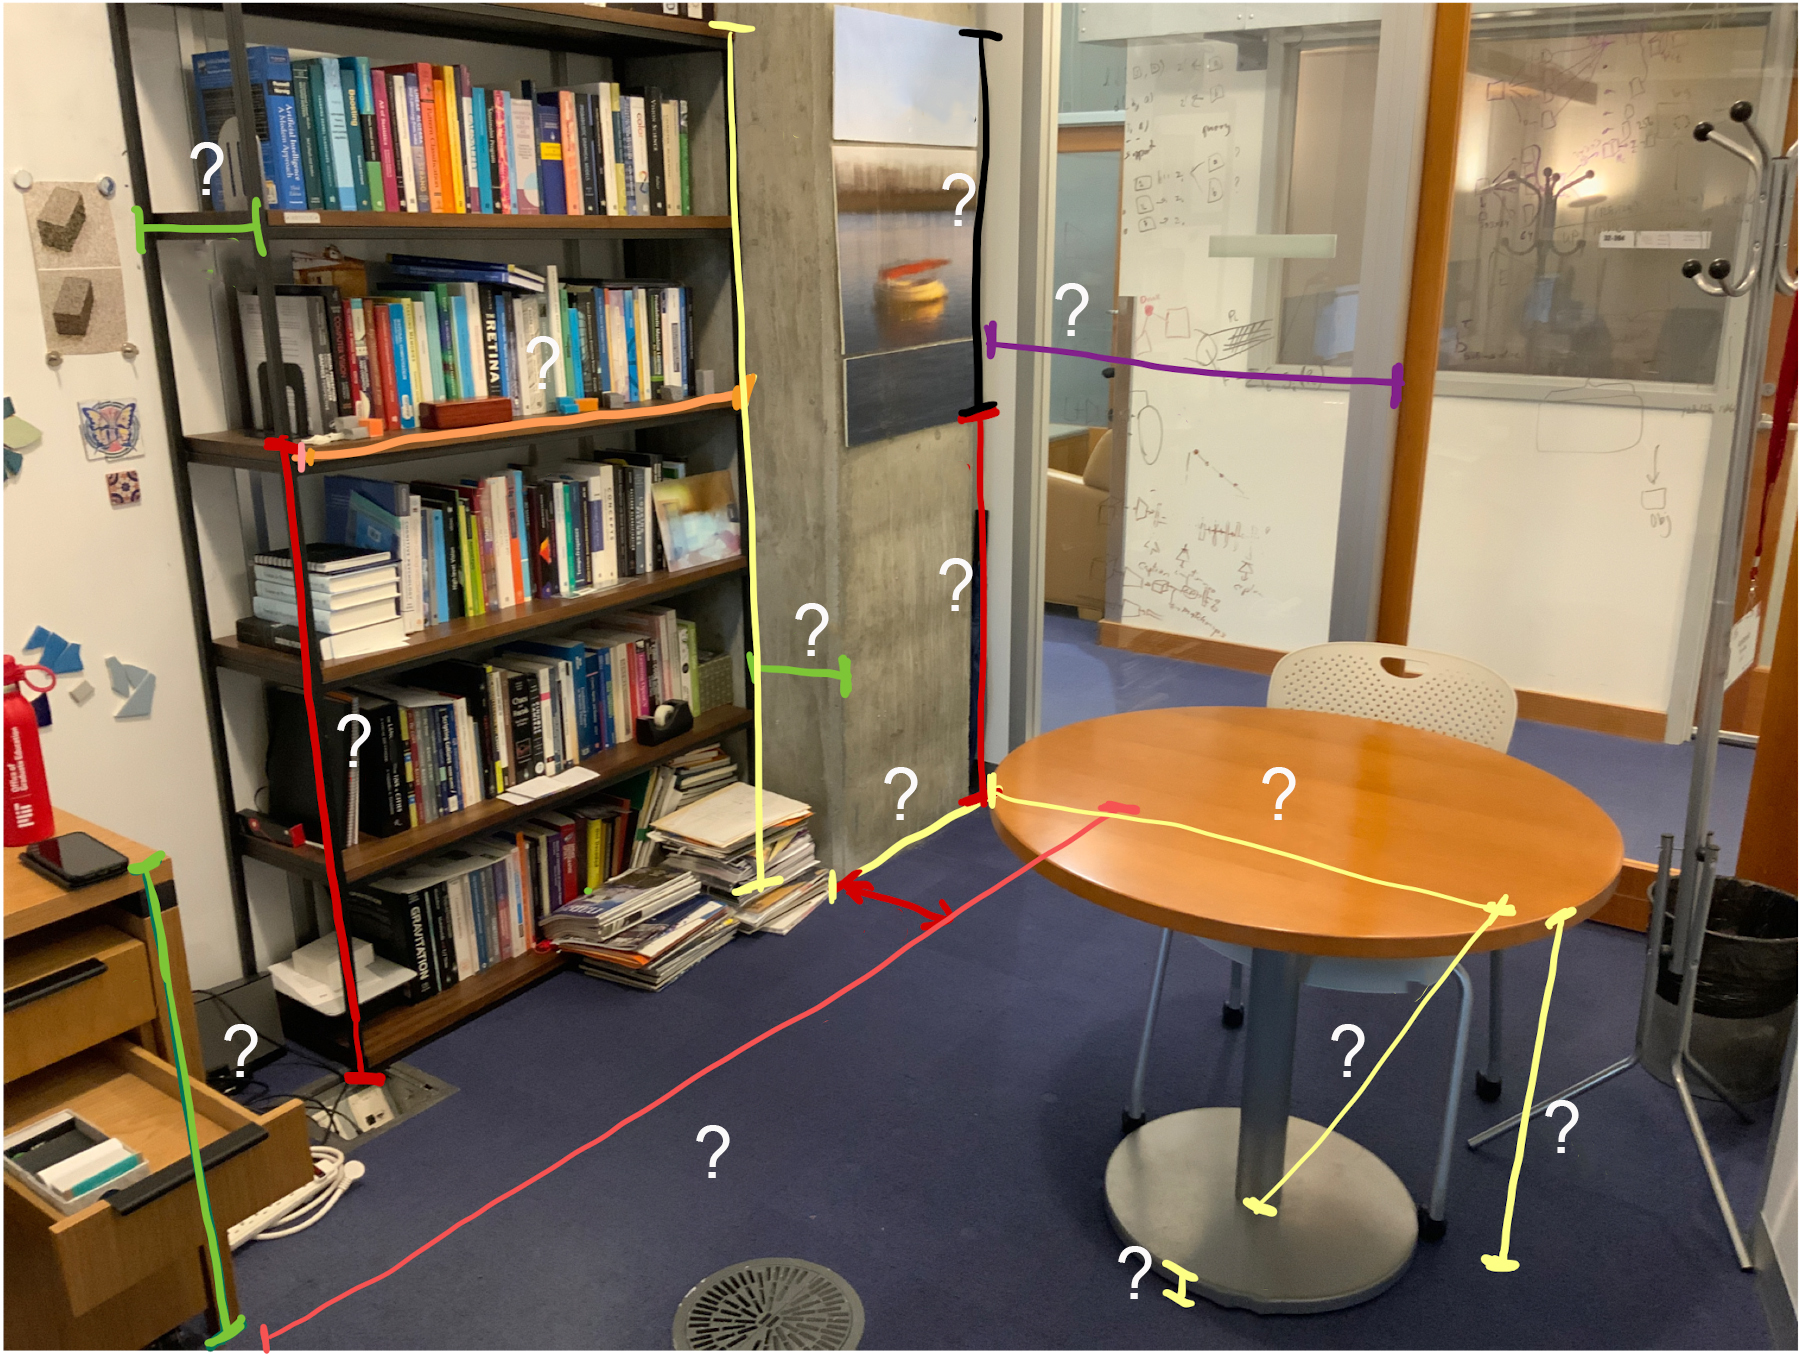
\includegraphics[width=.8\linewidth]{figures/single_view_3d/inverse_office_measurements.jpg}
}
\caption{Is it possible to recover three-dimensional (3D) scene information from a single two-dimensional (2D) image? How tall is the desk? How wide is the bookshelf? What do we need to know about the scene in order to be able to answer those questions?}
\label{fig:finding_depth_office}
\end{figure}


%The goal of this chapter is to introduce the reader to the principles of single view metrology.

Single view metrology relies on understanding the geometry of the image formation process, the rules of perspective, and other visual cues present in the image to answer questions about the 3D structure of the scene. This is in contrast to other methods, like stereo vision, structure from motion or multiview geometry, which utilize multiple images to reconstruct 3D information. The reader should consult specialized monographs for a deeper analysis such as the book on multiview geometry by Hartley and Zisserman \cite{Hartley2004}. 

%For instance, Zisserman, Faugeras, ... Criminisi work.


%Our goal is, given a single photograph, like the picture of the office we used before (\fig{\ref{fig:finding_depth_office}}), can we estimate 3D measurements using only a single 2D image captured by the camera? 


There are many scenarios where recovering 3D information from a single view is important. There are applications from which only one view is available, such as when looking at paintings or TV, when analyzing photographs, and so on. Even when we have stereo vision, stereo is only effective when the disparity is large enough which limits the range of distances for which stereo can be used reliably.

We could just start by diving into learning-based methods and train a huge neural network to solve the task, but that would be no fun (we will do it later, no worries). Instead, we will start by using a model based single-view metrology. There will be no learning involved. Instead we will derive cues for 3D estimation from first principles.  


\section{A Few Notes about Perception of Depth by Humans}

%3D human perception is so powerful, it does not need semantics, it does not even need stereo vision. 
The image in \fig{\ref{fig:streetgeons}}, recreated from Mezzanotte and Biederman \cite{Biederman1976}, displays a flat set of lines that elicit a powerful 3D perception. Even more striking is that we perceive far more than mere 3D geometric figures (which is already intriguing, considering we are looking at a flat piece of paper). We discern buildings, people, a car in the street, the sky between the structures, and even what appears to be the entrance to a movie theater on the left sidewalk. Yet, the sidewalk is simply one line!

\begin{figure}[!h]
\centerline{
\includegraphics[width=.8\linewidth]{figures/single_view_3d/streetgeons.eps}
}
\caption{The image shows how scene understanding is possible from simple 3D cues and context. This sketch is a recreation of a real photograph shown in \cite{Biederman1976}. {\em Source}: 
Mezzanotte and Biederman.
% \cite{}.
}
\label{fig:streetgeons}
\end{figure}

%We can not shut it down, 
We  perceive everything we see in the sketch as 3D, even when we know that it's merely a 2D image. Our 3D processing is ingrained that we cannot easily switch off. That said, we are aware that it is just a collection of lines and geometric figures drawn on a flat piece of paper, but the 3D interpretation transforms the way in which we perceive the sketch. The influence of the 3D perceptual mechanisms is better appreciated when looking at visual illusions. 


3D visual illusions are remarkably powerful. One captivating 3D illusion is the {\bf Ames room}\index{Ames room}.

\marginnote{The Ames room was invented by Adelbert Ames, director of research at the Dartmouth Eye Institute, in 1946. Since then, illusions based on Ames' ideas have been utilized by comedians to create amusing effects.}[-1.2in]

The Ames room is an irregular room constructed in such a way that when you look at it with one eye from a particular vantage point, the room appears to be perfectly rectangular. This is achieved by making the part of the wall that is farther away from the viewer larger so that it appears fronto-parallel. 


\marginnote{Geometric description of the Ames room visual illusion.
\\[6pt]
\centerline{
\includegraphics[width=.4\linewidth]{figures/single_view_3d/ames_room_description.eps}
}
}[-.7in]

The best way to understand this illusion is by building it and experiencing it by yourself. You can find the instructions in \fig{\ref{fig:ames_room}}. When you look thought the aperture on the wall indicated by ``cut'' the room will appear square and smaller than it actually is, and it will seem as if you are looking inside the room from the middle of it despite that the opening is closer to the right wall. 


\begin{figure}[t]
\centerline{
\includegraphics[width=.8\linewidth]{figures/single_view_3d/ames_room.eps}
}
\caption{Make your own Ames room. Take a picture of this page and print it as large as you can (A4 or letter size will be sufficient). When you look through the aperture on the {\em front wall}, the room will appear square and smaller than it actually is. The shape of the {\em reference wall} is the only one that will appear unchanged, while all other planes will appear smaller than their actual size. You can change the room's content by drawing on the {\em reference wall} and then warping the image onto the other walls using homography. The floor pattern results from a homography with a square floor plan.}
\label{fig:ames_room}
\end{figure}


This illusion is especially remarkable when the room is large enough for people to walk in. You will notice that as people walk along the back wall, they appear to change in height. Your perception will disregard all of your (very strong) prior expectations about how that person should appear. \Fig{\ref{fig:ames_room_cat}} illustrates this phenomenon with our cut-out version of the Ames room.

\begin{figure}[t]
%\centerline{
%\includegraphics[width=.48\linewidth]%{figures/single_view_3d/ames_room_cat1.jpg}
%~
%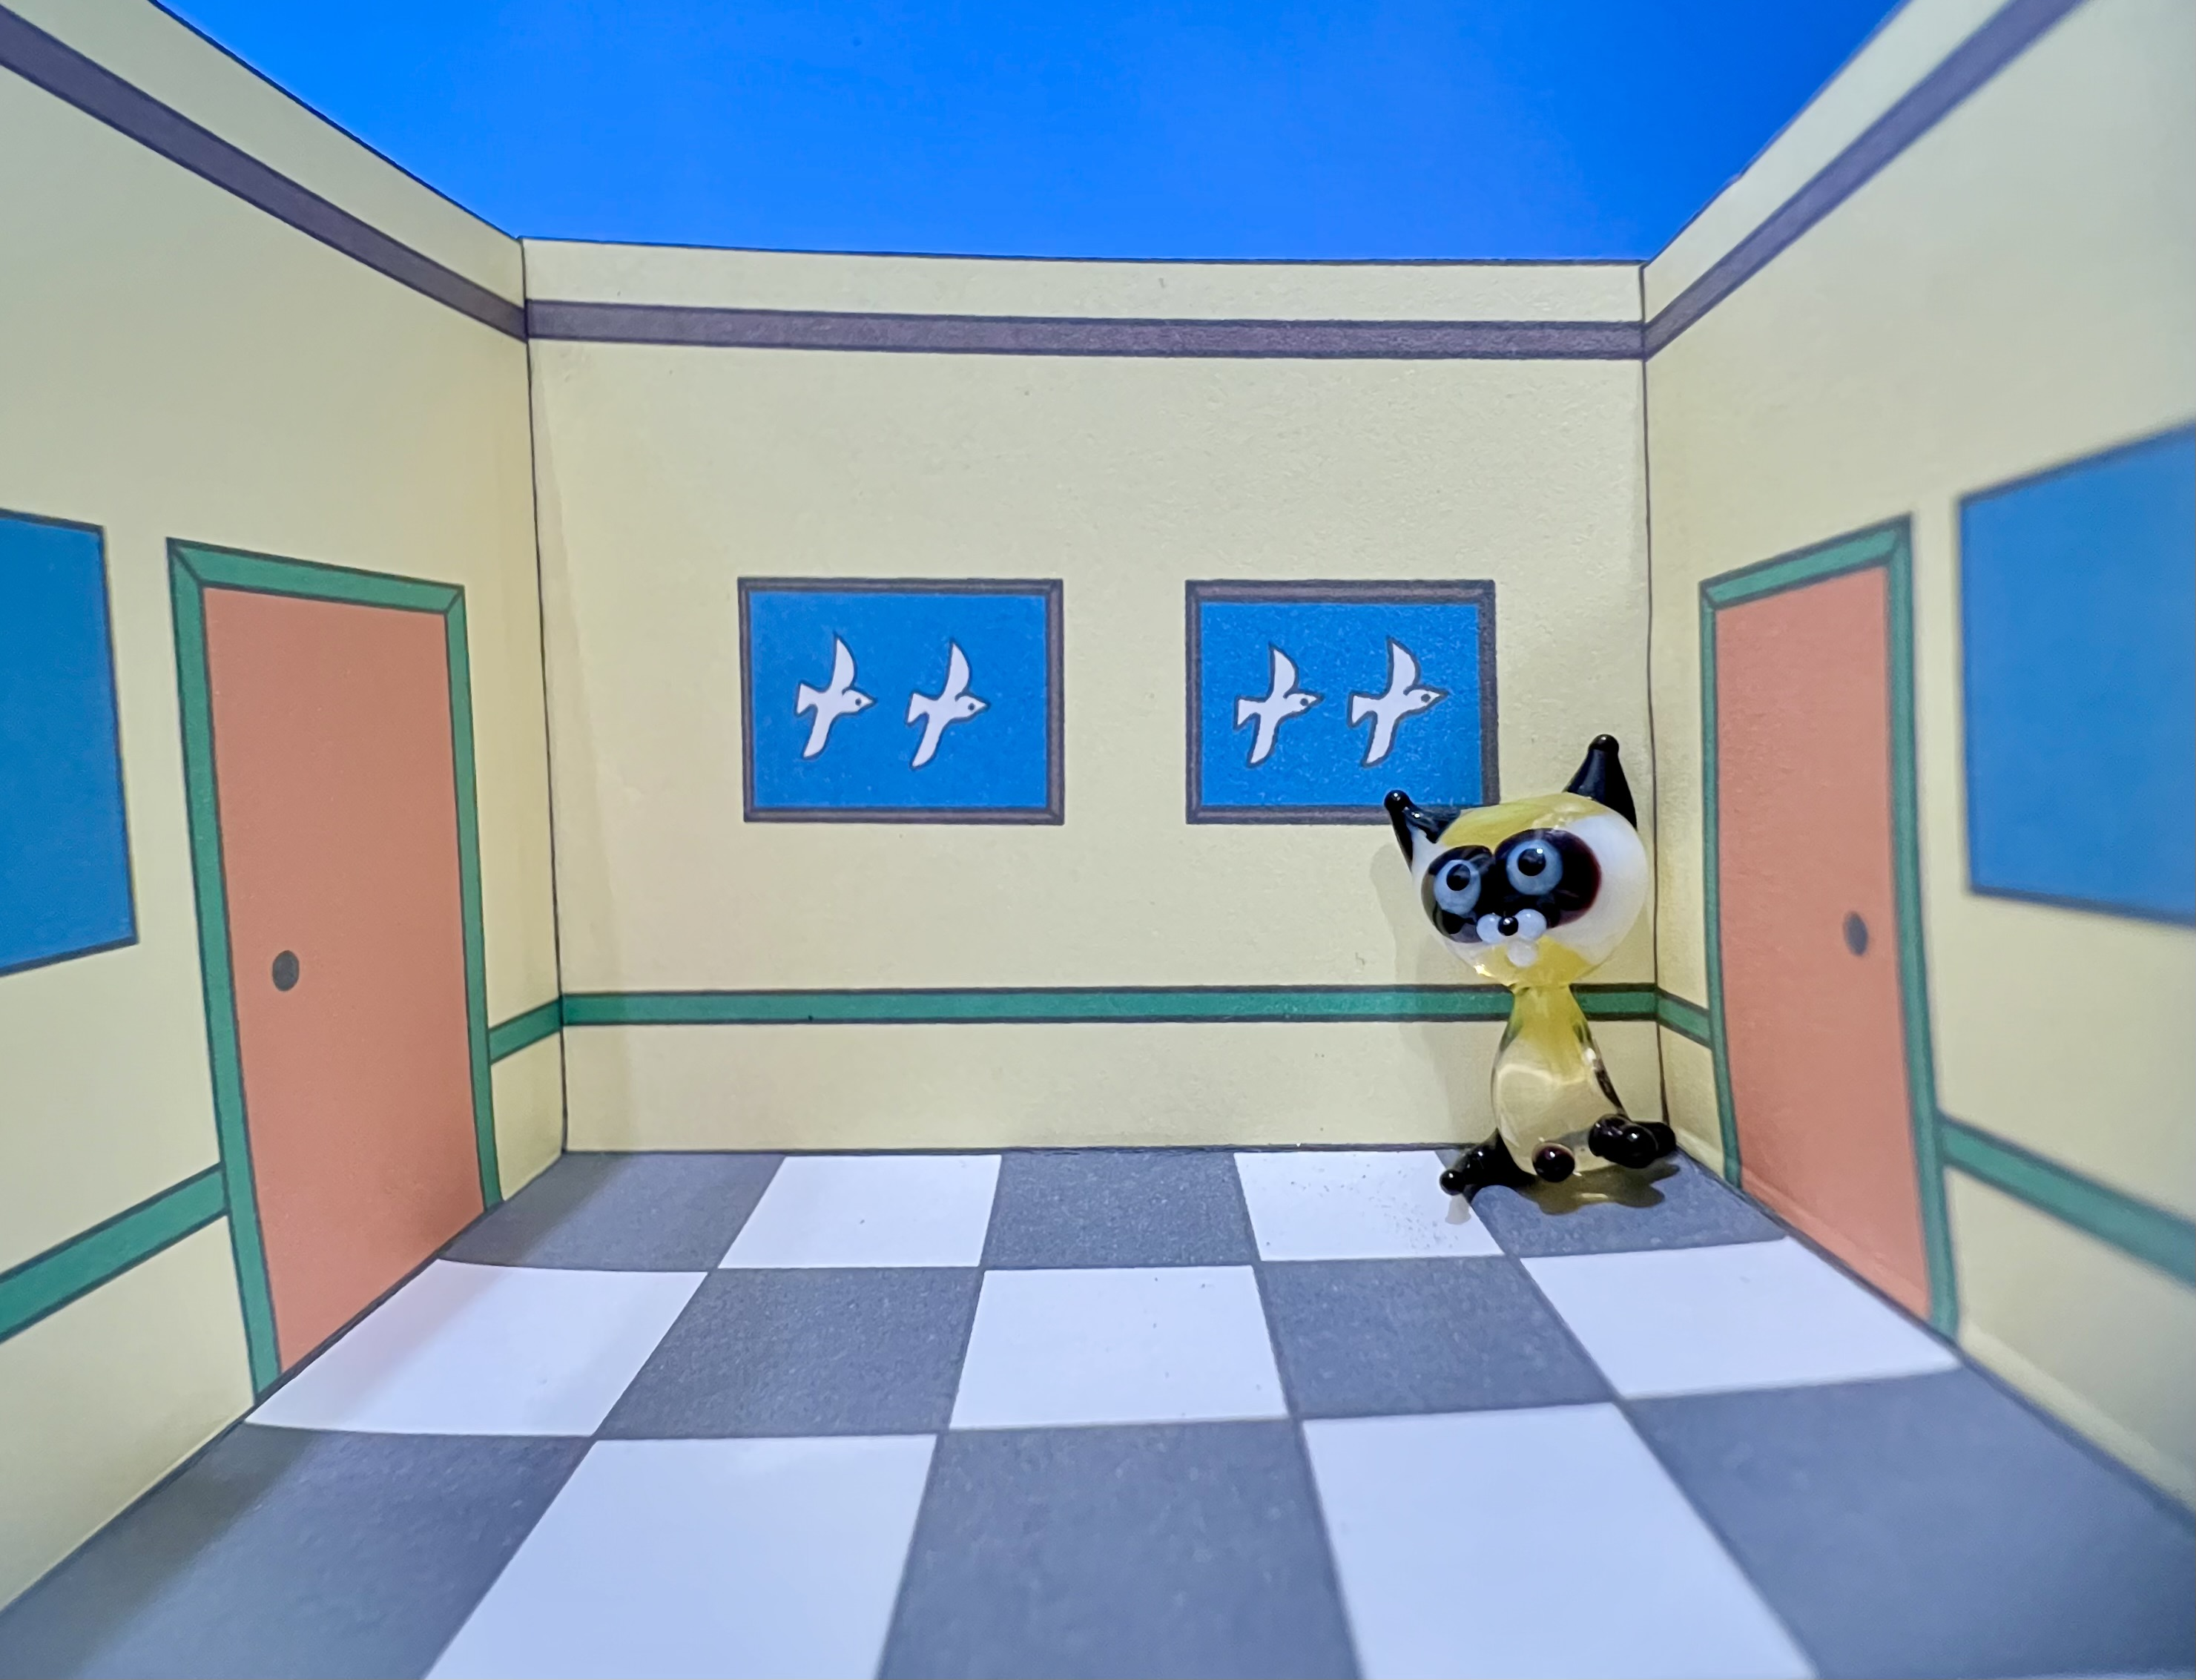
\includegraphics[width=.48\linewidth]{figures/single_view_3d/ames_room_cat2.jpg}
%}
\centerline{
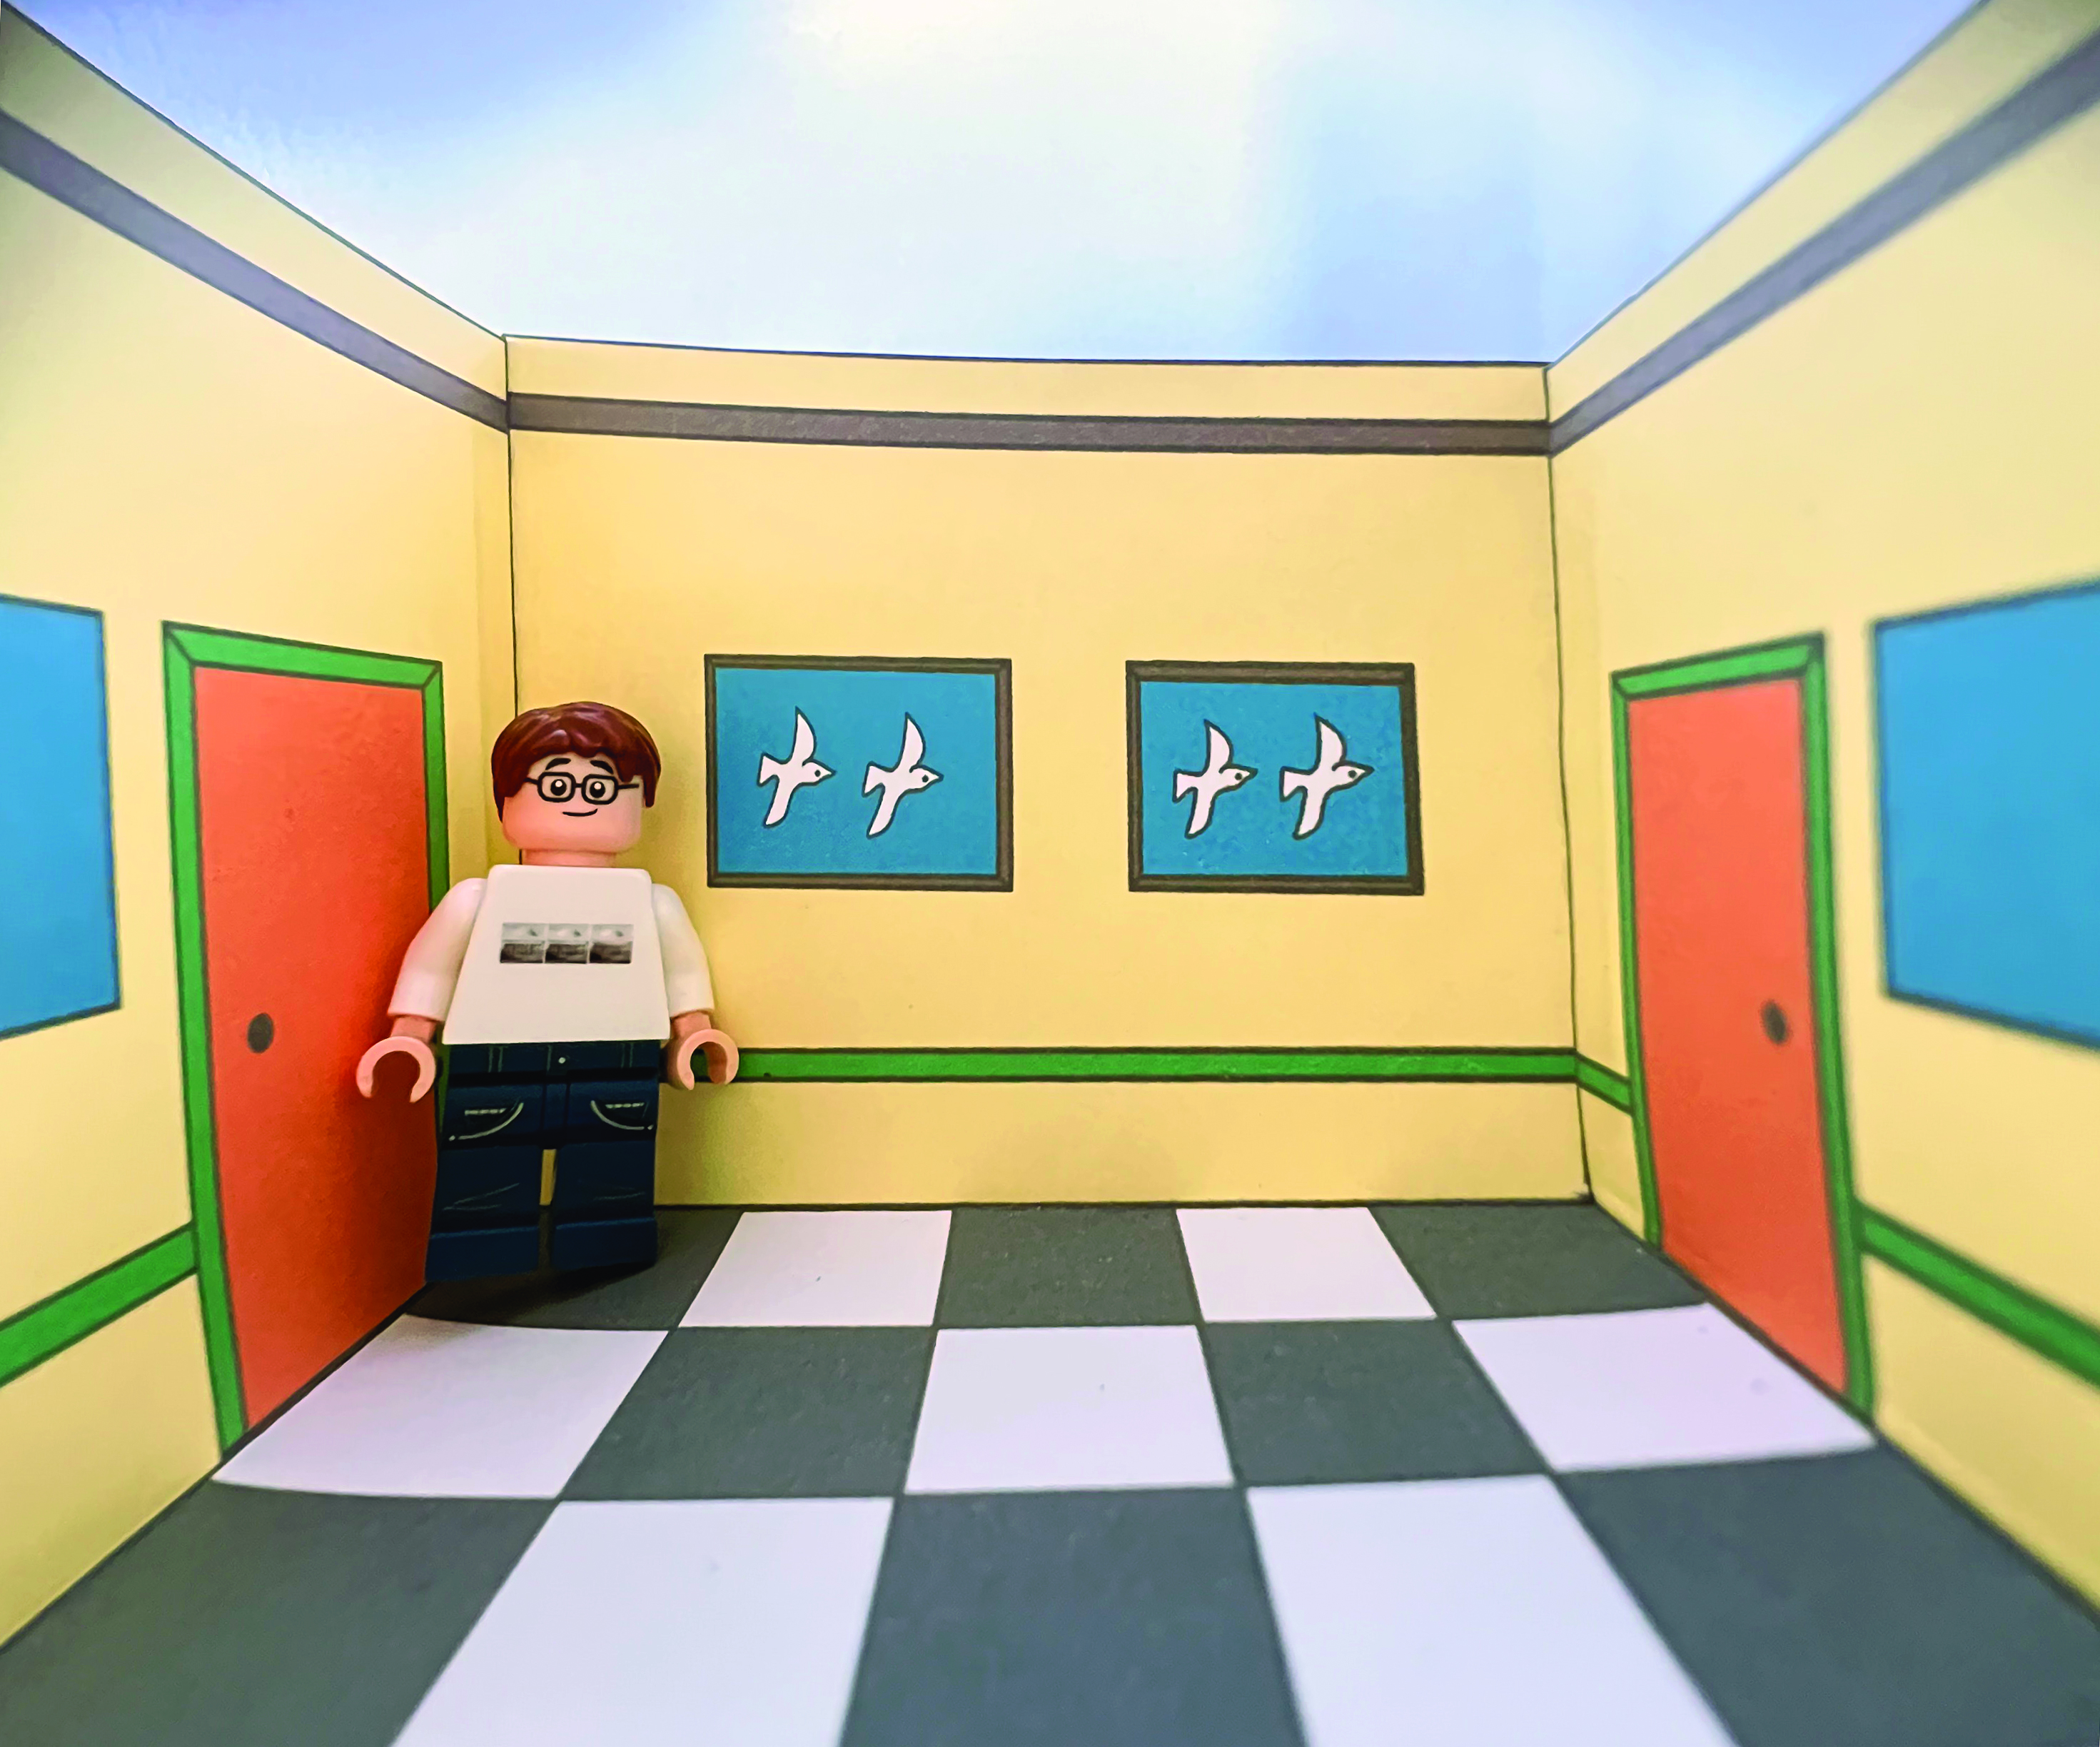
\includegraphics[width=.49\linewidth]{figures/single_view_3d/IMG_9148_small.jpeg}
~
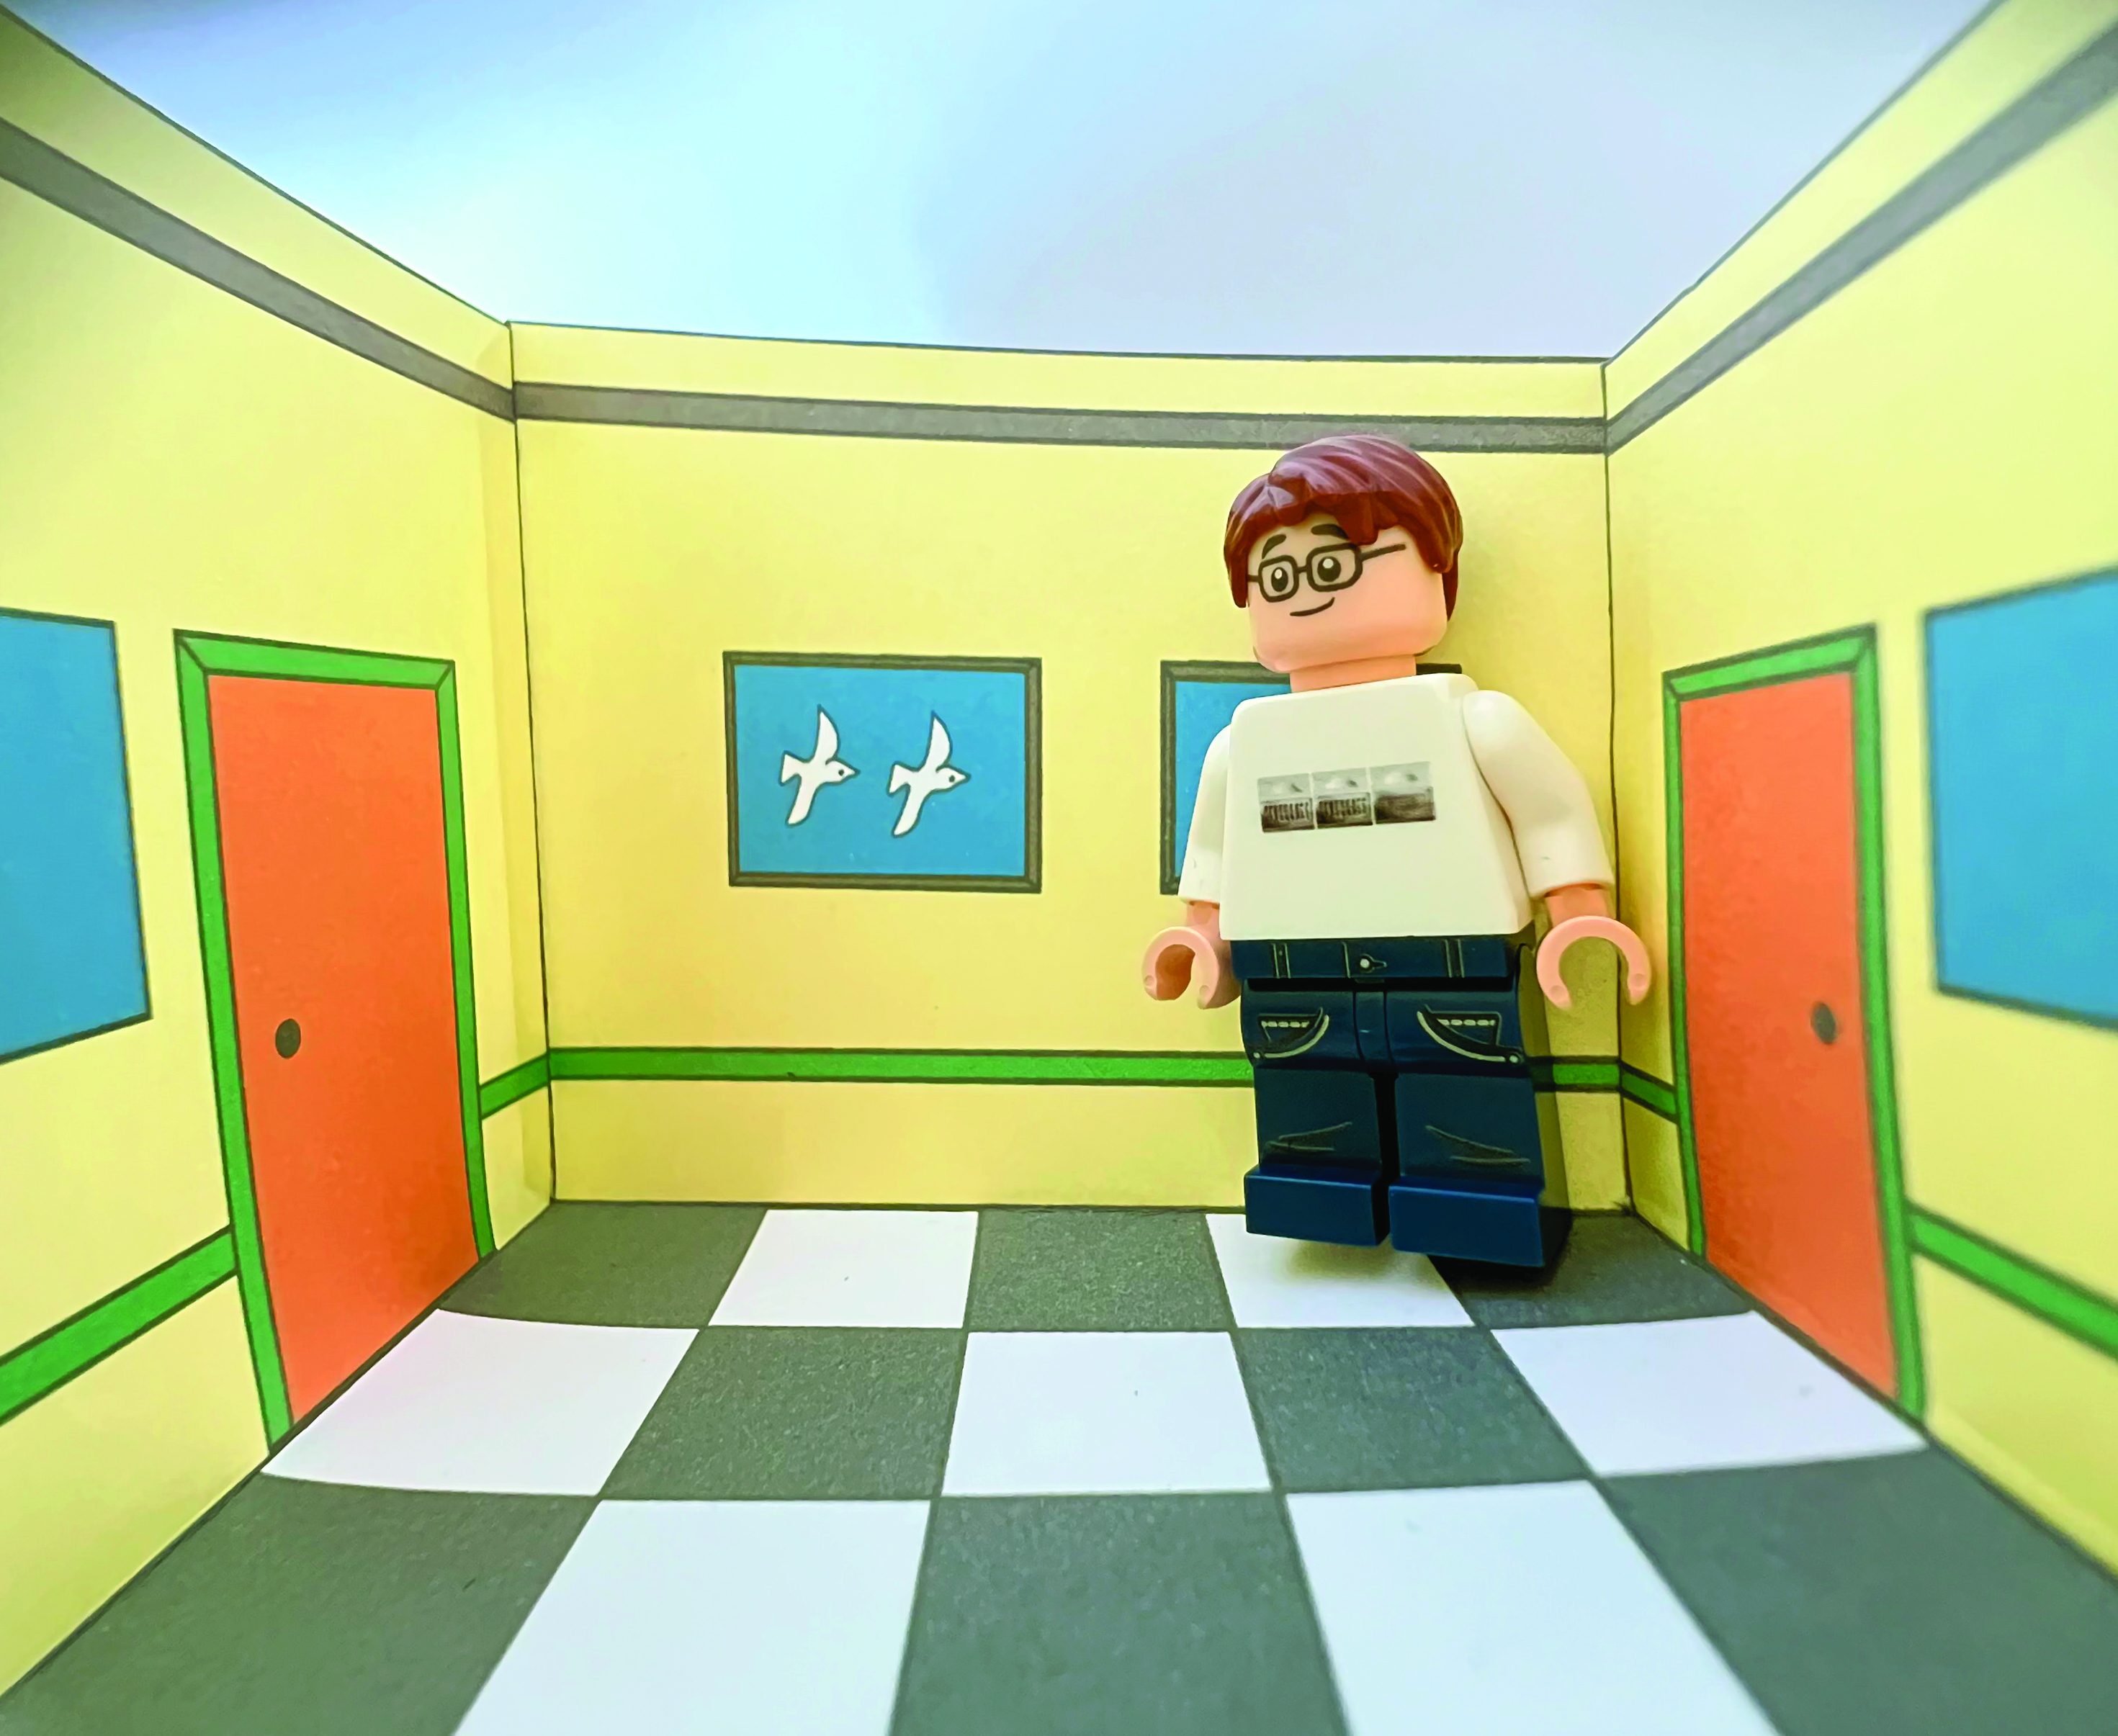
\includegraphics[width=.494\linewidth]{figures/single_view_3d/IMG_9150_large.jpeg}
}
\caption{If you place an object along the back wall of the Ames room shown in \fig{\ref{fig:ames_room}}, its perceived size will change. Also note that both doors appear to be similar en size despite being quite different in reality.}
\label{fig:ames_room_cat}
\end{figure}



\begin{comment}
Understanding the underlying principles is important to think about structural constraints one can impose on a neural architecture, but it is even more important when moving into unsupervised learning as, understanding the problem, can help thinking about appropriate unsupervised losses that can result in learning what we want. (MEGADEPTH IS ONE EXAMPLE)

\section{Monocular cues for depth perception}

make a list of all the cues, showing examples.
\end{comment}


Clearly, a single image contains very strong cues about the 3D scene structure. In the following sections we will study linear perspective, arguably the most powerful among all pictorial cues used for 3D interpretation from a 2D image.

\section{Linear Perspective}

Linear perspective uses parallel and orthogonal lines, vanishing points, the ground plane and the horizon line to infer the 3D scene structure from a 2D image. 
\marginnote{The discovery of linear perspective is attributed to the Italian architect Fillipo Brunelleschi in 1415.}

As we will see in the following sections, linear perspective relies on a few assumptions about the scene and, as a consequence, linear perspective is not a general cue that is useful in all scenes, but it is very powerful in most human-made environments. 

\subsection{Projection of 3D Lines}

In perspective projection, 3D lines project into 2D lines in the camera plane. Let's start writing the parametric vector form of a 3D line using heterogeneous coordinates. We can parameterize a 3D line with a point, $\mathbf{P}_0=[X_0, Y_0, Z_0]^\transpose$, and a direction vector, $\mathbf{D} = [D_X, D_Y, D_Z]^\transpose$, as:

\begin{equation}
\mathbf{P}_t = 
    \begin{bmatrix}
    X_0 + t D_x\\
    Y_0 + t D_y\\
    Z_0 + t D_z
    \end{bmatrix}
\label{eq:parametric_vector_line}
\end{equation}
The 3D point $\mathbf{P}_t$ moves along a line when the independent variable $t$ goes from $-\infty$ to $\infty$. A camera located in the world coordinates origin will observe a 2D line resulting from projecting the 3D line into the camera plane as shown in the sketch shown in \fig{\ref{fig:vanishing_points}}.

\begin{figure}
\centerline{
\includegraphics[width=1\linewidth]{figures/single_view_3d/vanishing_points.eps}
}
\caption{Projection of a 3D line onto the camera plane. The 3D line and the camera center form a plane (the camera center is a the world-coordinates origin). The intersection of this plane with the camera plane is the 2D line that appears in the image. The image point $\mathbf{v}$ is the vanishing point of the line.}
\label{fig:vanishing_points}
\end{figure}



We can get the equation of the 2D line that appears in the image by using the perspective projection equations, resulting in:
%\begin{eqnarray}
%x_t = f \frac{ X_0 + t D_X}{Z_0 + t D_Z} \\
%y_t = f \frac{ Y_0 + t D_Y}{Z_0 + t D_Z} \\
%\end{eqnarray}
%The 2D point $\mathbf{p}_t$
\begin{equation}
\mathbf{p}_t = 
    \begin{bmatrix}
    x_t\\
    y_t
    \end{bmatrix}
    =
    \begin{bmatrix}
    f \dfrac{ X_0 + t D_X}{Z_0 + t D_Z}\\[12pt]
    f \dfrac{ Y_0 + t D_Y}{Z_0 + t D_Z}
    \end{bmatrix}
\label{eq:line_projection}
\end{equation}

\marginnote{One subtle point about what is visible by the camera: Remember that when we plot the image plane we are using the virtual camera plane, but the real ``image'' is being formed behind the pinhole. So, in the example shown in \fig{\ref{fig:vanishing_points}}, the points along the line with positive $Z$-value might be visible even when they are behind the virtual camera plane.}

%We can do the same using homogeneous coordinates as we will see later. 

%The 3D line and the camera center form a plane. The intersection of this plane with the camera plane is the 2D line that appears in the image. 

%Observe that the 
%TODO: show this is the equation of a line.

\subsection{Vanishing Points}
\index{Vanishing point}

%~\\
Even though a line in 3D space extends infinitely, its 2D projection doesn't. According to \eqn{\ref{eq:line_projection}}, in the limit when $t$ goes to infinity, the line converges to a finite point called the vanishing point:
%\begin{eqnarray}
%\lim_{t \to \infty} x_t  & = & f \frac{D_X}{D_Z} = v_x\\
%\lim_{t \to \infty} y_t & = & f \frac{D_Y}{D_Z} = v_y
%\label{eq:vanishingpoint}
%\end{eqnarray}
\begin{eqnarray}
\mathbf{v} = \lim_{t \to \infty} \mathbf{p}_t =
\left [
\begin{array}{c}
    f \dfrac{D_X}{D_Z}\\[12pt]
    f \dfrac{D_Y}{D_Z}
    \end{array}
    \right ]
\label{eq:vanishingpoint}
\end{eqnarray}
The vanishing point, $\mathbf{v} = [v_x, v_y]^\transpose$, only depends on the direction vector, $\mathbf{D}$, thus all parallel lines in 3D project into non-parallel 2D images that converge to the same vanishing point in the image. If $D_Z = 0$ then the 3D line is parallel to the camera plane and the vanishing point is in infinite. 


\Fig{\ref{fig:vanishing_lines_and_planes}} shows a set of parallel 3D lines and their 2D image projections. Each group of parallel lines converges to a different vanishing point. Lines that are parallel to the camera plane remain parallel as they converge to a vanishing point in infinity. 

\begin{figure}[!h]
\centerline{
\includegraphics[width=1\linewidth]{figures/single_view_3d/vanishing_lines_and_planes.eps}
}
\caption{Parallel 3D lines converge to the same vanishing point. (a) The red lines are parallel to the optical axis and converge to a vanishing point in the center. (b) Two sets of parallel lines contained in an horizontal plane, parallel to the optical axis. Their vanishing points are on an horizontal image line.}
\label{fig:vanishing_lines_and_planes}
\end{figure}

All the sets of parallel lines inside a plane converge to a set of co-linear vanishing points. These points lie along the plane's horizon line.

Vanishing points are very useful to recover the missing depth of the scene as we will see later. The human visual system also makes use of vanishing points for 3D perception. Take, for example, the {\em leaning tower visual illusion} \cite{Kingdom2017} as depicted in \fig{\ref{fig:LeaningTower1}}. Here, a pair of identical images of the Leaning Tower of Pisa are placed side by side. Interestingly, despite being identical, they create an illusion of leaning with different angles. The image on the right appears to have a greater tilt than the one on the left. One explanation of this illusion is that the lines of each tower converge at a different vanishing point. If both towers were parallel in 3D, all the lines would converge to the same 2D vanishing point. As they do not, our brain interprets that the towers should have different 3D orientations. This process is automatic and we can not shut it down despite the fact that we know both images are identical.


\begin{figure}[t]
\centerline{
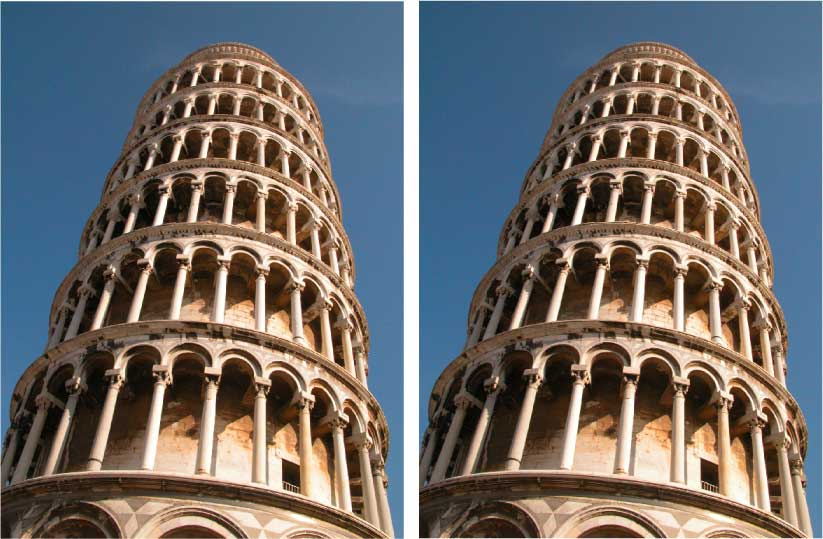
\includegraphics[width=1\linewidth]{figures/single_view_3d/LeaningTower1.jpg}
}
\caption{The {\em leaning tower illusion} \cite{Kingdom2017} involves two identical pictures placed side by side. The picture on the right appears to be more tilted than the one on the left.}
% http://www.scholarpedia.org/article/Leaning_tower_illusion
% Kingdom, F. A. A., Yoonessi, A. & Gheorghiu, E. (2007). The Leaning Tower illusion: a new illusion of perspective. Perception, 36, 475-477. 
\label{fig:LeaningTower1}
\end{figure}


%\subsection{Vanishing point using homogenous coordinates}

%Let's now derive the formulation to compute the vanishing point of a line. If we have arbitrary extrinsic and intrinsic camera parameters, we can write the vanishing point in homogeneous coordinates as:

Homogeneous coordinates offer an alternative way of working with vanishing points. Let's start by writing the parametric vector form of a 3D line using homogeneous coordinates:
\begin{equation}
\mathbf{P}_t = 
    \begin{bmatrix}
    X_0 + t D_X\\
    Y_0 + t D_Y\\
    Z_0 + t D_Z\\
    1
    \end{bmatrix}
    =
    \begin{bmatrix}
    X_0/t + D_X\\
    Y_0 /t+ D_Y\\
    Z_0/t + D_Z\\
    1/t
    \end{bmatrix}
\label{eq:parametric_vector_line_homogeneous}
\end{equation}
The first term is equivalent to the writing of the line in \eqn{\ref{eq:parametric_vector_line}}. As homogeneous coordinates are invariant to a global scaling, we can divide the vector by $t$ which results in the second equality.

In the limit $t \to \infty$ the fourth coordinate of \eqn{\ref{eq:parametric_vector_line_homogeneous}} converges resulting in:
\begin{equation}
    \mathbf{P}_\infty = 
    \begin{bmatrix}
    D_X\\
    D_Y\\
    D_Z\\
    0
    \end{bmatrix}
    = 
    \begin{bmatrix}
    \mathbf{D}\\
    0
    \end{bmatrix}
\end{equation}
Note that here we are representing a point at infinity with finite homogeneous coordinates. This is another of the advantages of homogeneous coordinates. \marginnote{Homogeneous coordinates allow us to represent points at infinity with finite coordinates by setting the last element to 0.} 

The vanishing point, in homogeneous coordinates, is the result of projecting $\mathbf{P}_\infty$ using the camera model, $\mathbf{M}$:
\begin{equation}
    \mathbf{v} = 
    \mathbf{M} 
    \mathbf{P}_\infty 
    = 
    \mathbf{K} 
    \begin{bmatrix}
    \mathbf{R} & \mathbf{T} 
    \end{bmatrix}
    \begin{bmatrix}
    \mathbf{D}\\
    0
    \end{bmatrix}
    = 
    \mathbf{K} \mathbf{R} \mathbf{D}
\label{eq:vanishing_projection}
\end{equation}
The last equality is obtained by using \eqn{\ref{eq:extrinsic}}, and it shows that the vanishing point coordinates do not depend on camera translation. Only a camera rotation will change the location of the vanishing points in an image. If a scene is captured by two identical cameras translated from each other, their corresponding images will have the same vanishing points. 

Both \eqn{\ref{eq:vanishingpoint}} and \eqn{\ref{eq:vanishing_projection}}
are equivalent if we replace $\mathbf{K}$ by the appropriate perspective camera model.
 
If instead of perspective projection, we have parallel projection, then all the vanishing points will project at infinity in the image plane. 



\subsection{Horizon Line}
%~\\
\index{Horizon line}


Any 3D plane becomes a half-plane in the image and has an horizon line. The horizon line is the line that passes by all the vanishing points of all the lines contained in the plane as shown in \fig{\ref{fig:palma_horizon}}.



\begin{figure}
\centerline{
%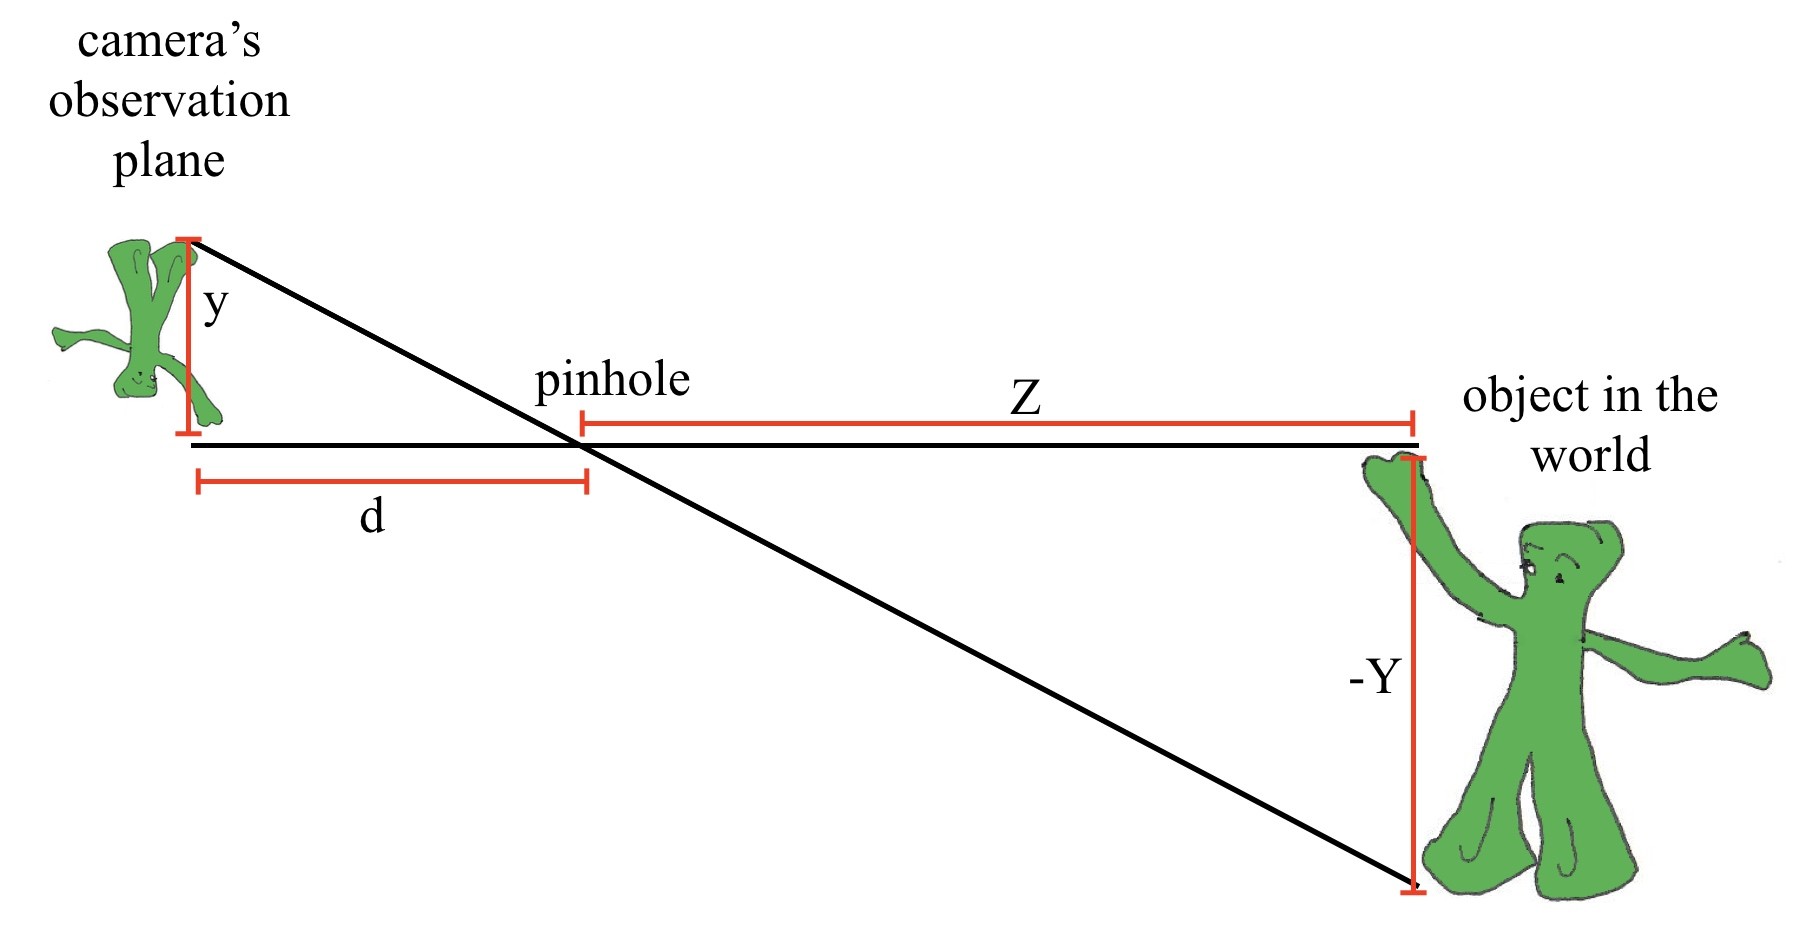
\includegraphics[width=.8\linewidth]{figures/imaging/pinholeGeomGumby.jpg}
\includegraphics[width=1\linewidth]{figures/single_view_3d/palma_horizon.png}
}
\caption{All parallel lines contained in a plane converge to a set of vanishing points. All those vanishing points are contained in the {\bf horizon line} of the plane. Parallel planes have the same horizon line.}
\label{fig:palma_horizon}
\end{figure}

As parallel lines converge to the same vanishing point, parallel planes also have the same horizon line. In \fig{\ref{fig:palma_horizon}}, the lines in the building facade that are parallel to the ground also converge to a vanishing point that lies on the horizon line. In this particular examples, the lines in the facade also happen to be parallel to one of the axis of the floor tiles, converging to the same vanishing point on the right side of the figure.


The ground plane is a special plane because it supports most objects. This is different than a wall. Both are planes, but the ground has an ecological importance that a wall does not have. The point of contact between objects and the ground plane informs about its distance. The distance between the contact point and the horizon line is related to distance between the object and the camera. Objects further away have a contact point projecting onto a higher point in the image plane. 


%\fig{\ref{fig:horizon_line_cross_products}} illustrates an application of describing points and lines with homogeneous coordinates  to compute the horizon line in an image given the equations of four lines in a plane. 

\Fig{\ref{fig:horizon_line_cross_products}} illustrates how to detect the horizon line using homogeneous coordinates.
If lines $\boldsymbol{l}_1$ and $\boldsymbol{l}_2$, in homogeneous coordinates, correspond to the 2D projection of 3D parallel lines, we can obtain the vanishing point as their intersection (cross-product, $\boldsymbol{l}_1 \times \boldsymbol{l}_2$). If we now have another set of parallel lines, contained in the same plane, $\boldsymbol{l}_3$ and $\boldsymbol{l}_4$, we can get another vanishing point by computing their cross-product. Finally, the horizon line is the line that passes through both points that can be computed as the cross-product of the vanishing points in homogeneous coordinates. 


\begin{figure}
\centerline{
%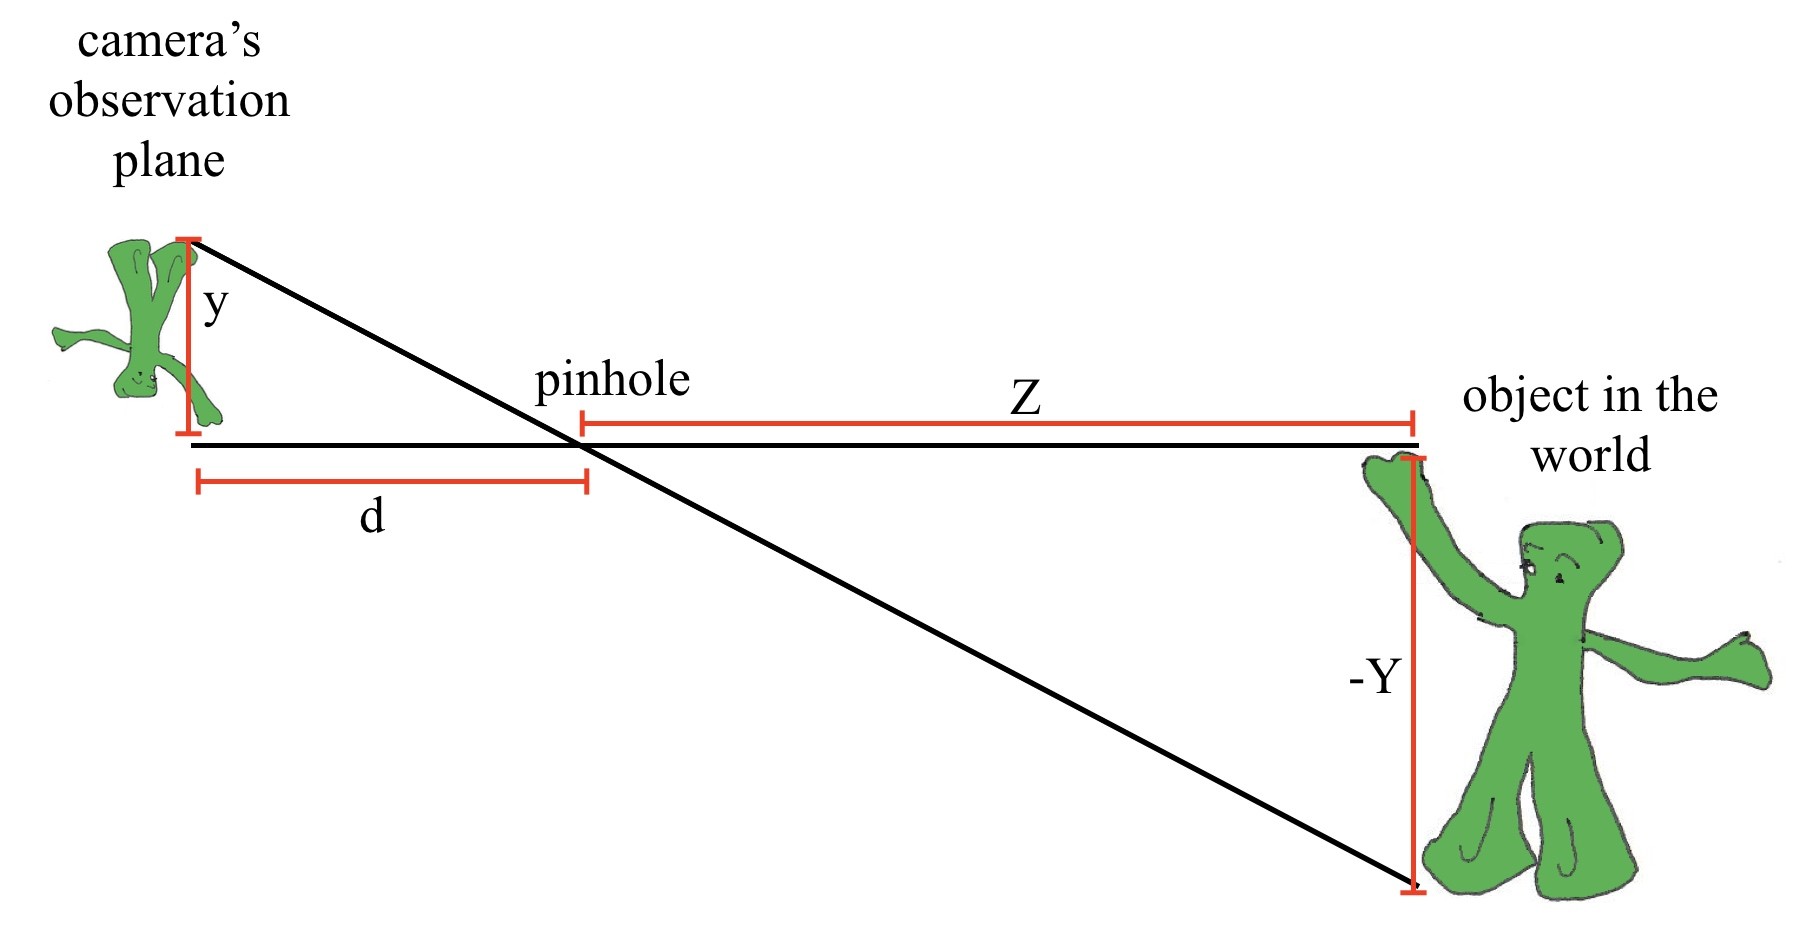
\includegraphics[width=.8\linewidth]{figures/imaging/pinholeGeomGumby.jpg}
\includegraphics[width=.9\linewidth]{figures/imaging_geometry/horizon_line.eps}
}
\caption{Using parallel lines, in homogeneous coordinates, to compute vanishing points and the horizon line.}
\label{fig:horizon_line_cross_products}
\end{figure}

\subsection{Detecting Vanishing Points}

\Fig{\ref{fig:vanishing_lines}} shows the office scene and three vanishing points computed manually. In this scene there are three dominant orientations along orthogonal directions. The three vanishing points are estimated by selecting pairs of long edges in the image corresponding to parallel 3D lines in the scene and finding their intersection. 

\begin{figure}
\centerline{
%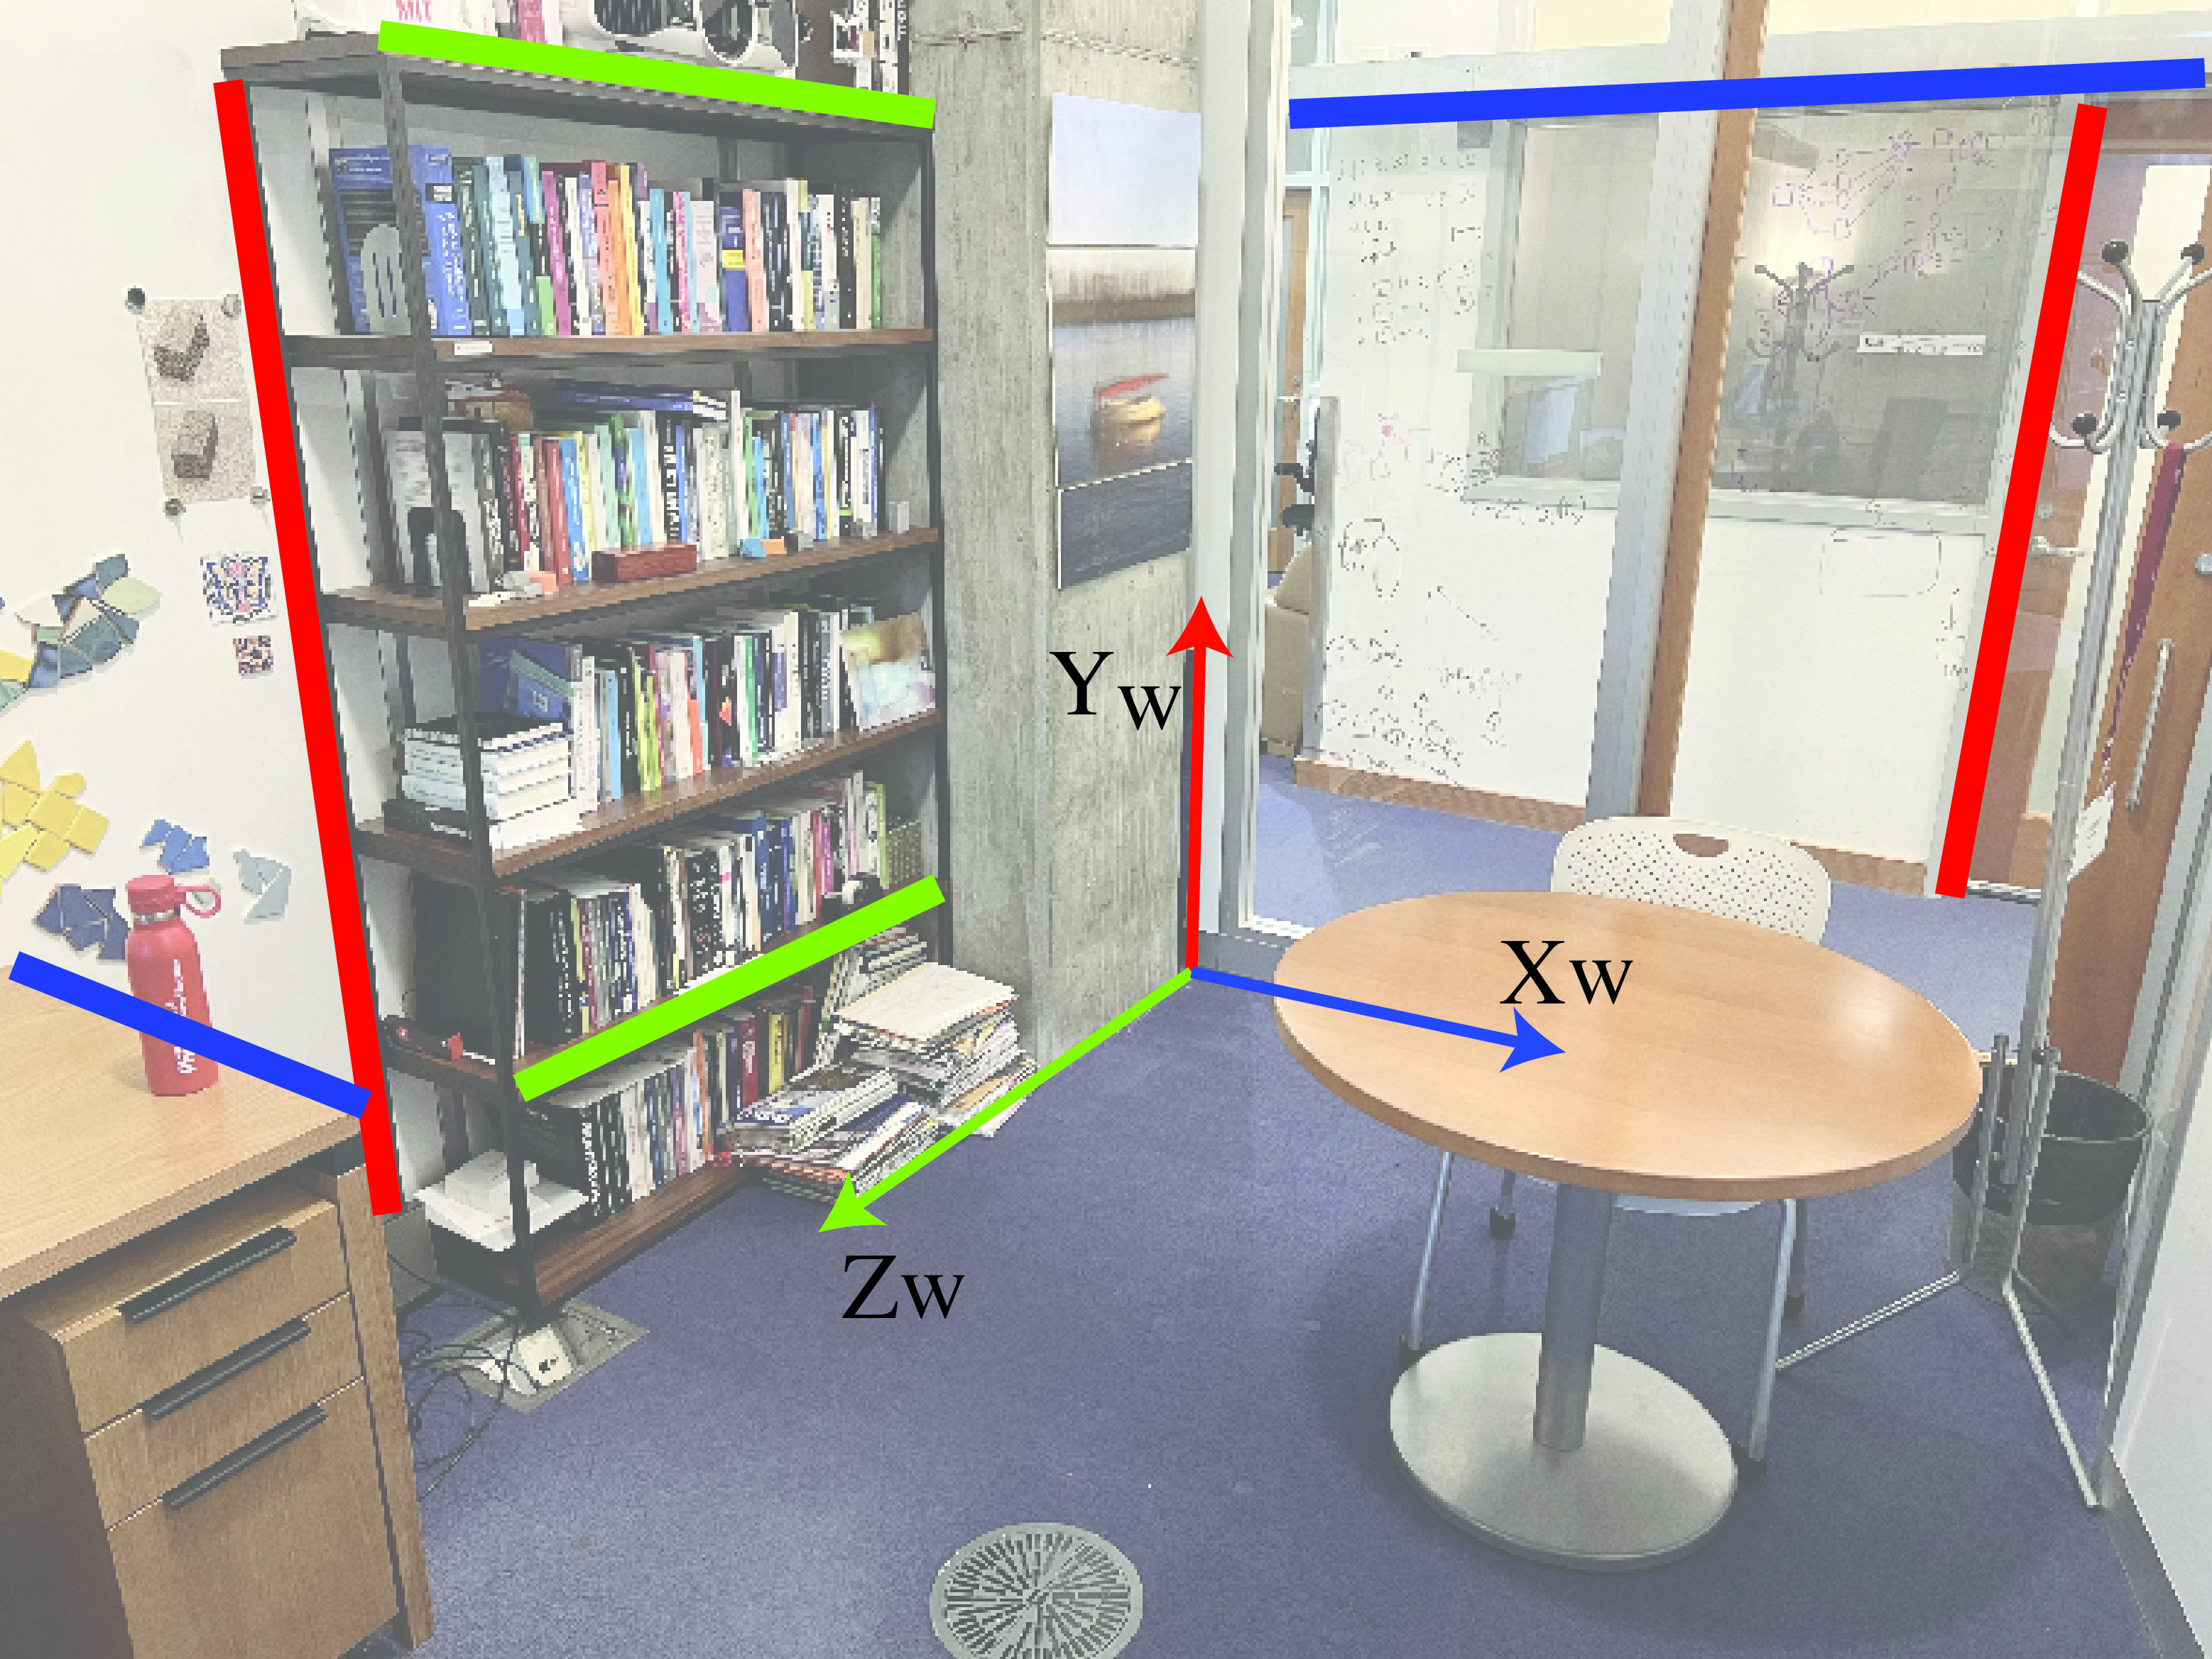
\includegraphics[width=.65\linewidth]{figures/single_view_3d/parallel_lines_in_3D.eps}
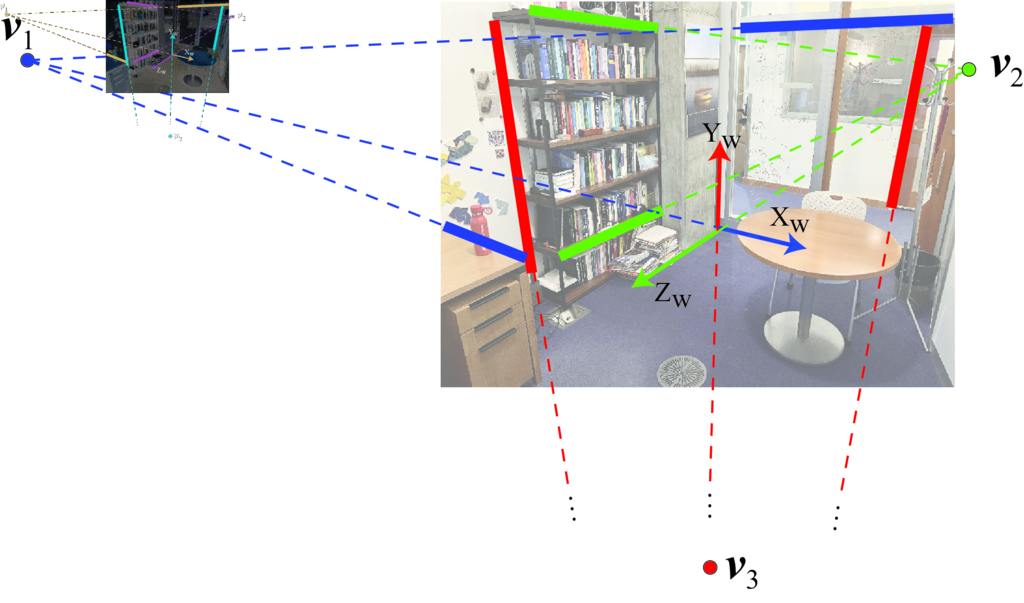
\includegraphics[width=1\linewidth]{figures/single_view_3d/office_vanishing_points_3.eps}
} 
\caption{Most object boundaries in this photograph are oriented parallel to one of the world-coordinates reference frame (the world-coordinates frame is chosen in this way on purpose). All the parallel 3D lines converge on the image plane in a vanishing point. In this picture there are three main vanishing points, each of them related to one of the world-coordinates frame.}
\label{fig:vanishing_lines}
\end{figure}

Vanishing points can be extracted automatically from images by first detecting image edges and their orientations (like we did in \chap{\ref{chapter:simplesystem}}) and then using RANSAC (\sect{\ref{sec:RANSAC}}) to group the edges: every pair of edges will vote for a vanishing point and the point with the largest support will be considered a vanishing point. 

There are also learning-based approaches for vanishing point detection using graphical models \cite{coughlan1999manhattan}, or deep learning based approaches such as DeepVP \cite{Chang2018DeepVPDL} and NeurVPS \cite{zhou2019neurvps}.



%https://www.microsoft.com/en-us/research/wp-content/uploads/2016/02/criminisi_dagm2002.pdf

%\subsection{Measuring with planes}
\begin{comment}

\subsection{Cross-ratio}

1- description of cross ratio 

2- figure showing 4 lines...

3- a picture with a metric tape and illustrate the cross-ration with an example

4- explain what happens when one of the points goes to infinity. This is useful when we know when a vanishing point is. 
\end{comment}


\section{Measuring Heights Using Parallel Lines}

%A wonderful manuscript about \cite{criminisi1999accurate}

Let's now use what we have seen up to now to measurement distances in the world from a single image. We will discuss in this section how to make those measurements using three vanishing points, or just the horizon line and one vanishing point. We will not use camera calibration or the projection matrix. For a deeper analysis we refer the reader to the wonderful thesis of A. Criminisi \cite{criminisi1999accurate}.


%We will need a reference measure. If you do not have one, then we can select to point in the scene and define the distance between them as 1. Then all the other measurements will be relative to that. 

%Single view metrology
%- show office example and recover some measurements.

%Lets start inferring distances in the ground plane. 

%Note that all of those measurements can be extracted without needing the camera intrinsic parameters. Information is propagated from one point to another via parallel 3D lines and cross-ratios. 

Before we can make any 3D measurements we need to study an important invariant of perspective projection: the cross-ratio.

\subsection{Cross-Ratio}

As we have discussed before, perspective projection transforms many aspects of the 3D world when projecting into the 2D image: angles between lines are not preserved, the relative lengths between lines is not preserved, parallel 3D lines do not project into 2D parallel lines in the image (unless they are also parallel to the camera plane), and so on. Fortunately, some geometric properties are preserved under perspective projection. For instance, straight lines remain straight. Are there other quantities that are preserved? The cross-ratio is one of those quantities. 


The cross-ratio of four collinear points is defined by the expression:
\begin{equation}
CR \left( \mathbf{P}_1,\mathbf{P}_2,\mathbf{P}_3,\mathbf{P}_4 \right) 
= 
\frac{\left| \mathbf{P}_3 -\mathbf{P}_1 \right| \left|\mathbf{P}_4 -\mathbf{P}_2 \right|}
{\left| \mathbf{P}_3 -\mathbf{P}_2 \right| \left|\mathbf{P}_4 -\mathbf{P}_1 \right|}
\end{equation}
where $\left| \mathbf{P}_i -\mathbf{P}_j \right|$ is the euclidean distance between points $\mathbf{P}_i$ and $\mathbf{P}_j$, using heterogeneous coordinates. 

%\marginnote{
\centerline{
\includegraphics[width=.25\linewidth]{figures/single_view_3d/4_colinear_points.eps}
}
%}

The cross-ratio is considered the most important projective invariant. Two sets of points $\mathbf{P}$ and $\mathbf{Q}$ related by a projective transformation, as shown in \fig{\ref{fig:cross_ratio_description}}, have the same cross-ratio (regardless of the choice of origin $\mathbf{O}$ or scale factor). That is:
\begin{equation}
CR(\mathbf{P}_1,\mathbf{P}_2,\mathbf{P}_3,\mathbf{P}_4) = CR(\mathbf{Q}_1,\mathbf{Q}_2,\mathbf{Q}_3,\mathbf{Q}_4)
\end{equation}


\begin{figure}
\centerline{
\includegraphics[width=.9\linewidth]{figures/single_view_3d/cross_ratio_description2.eps}
} 
\caption{The set of points $\mathbf{P}$ are related to the points $\mathbf{Q}$ (and $\mathbf{R}$) by the cross-ratio. The point $\mathbf{R}_1$ is in infinity because the line connecting the points $\mathbf{R}$ is parallel to the line passing by $\mathbf{O}$, $\mathbf{P}_1$, and $\mathbf{Q}_1$.}
\label{fig:cross_ratio_description}
\end{figure}

The order in which these points are considered matters in the calculation. There are $4!=24$ possible orderings resulting in six different values. If two sets of points, related by a projection, have the same ordering, then their cross ratio will be preserved. We do not provide the proof for the cross-ratio invariant here. 

When one of the points is at infinity, all the terms that contain that point are cancelled out (this can also be seen by taking a limit). In the case of the points $\mathbf{R}$ from \fig{\ref{fig:cross_ratio_description}} we get that cross-ratio is:
\begin{equation}
CR(\mathbf{R}_1,\mathbf{R}_2,\mathbf{R}_3,\mathbf{R}_4) = 
\frac{\left| \mathbf{R}_4 -\mathbf{R}_2 \right| }
{ \left| \mathbf{R}_3 -\mathbf{R}_2 \right|}
\end{equation}
This value is equal to the cross-ratio of the points $\mathbf{P}$ and $\mathbf{Q}$.

To gain some intuition about the cross-ratio invariant, let's look at an empirical demonstration. \Fig{\ref{fig:cross_ratio_rulers}} shows a ruler seen under different view points. The blue dots correspond to same ruler locations with $P_1=0$ in, $P_2=6$ in, $P_3=8$ in, and $P_4=10$ in (we are making these measurements in inches, but note that the units do not affect the cross-ratio as it is scale invariant). Using those measurements, the cross-ratio is: $(8 \times 4)/(2 \times 10) = 1.6$. The same cross-ratio is obtained if we measure the positions of the four points using image coordinates and measuring distances in the image plane.

\begin{figure}
\centerline{
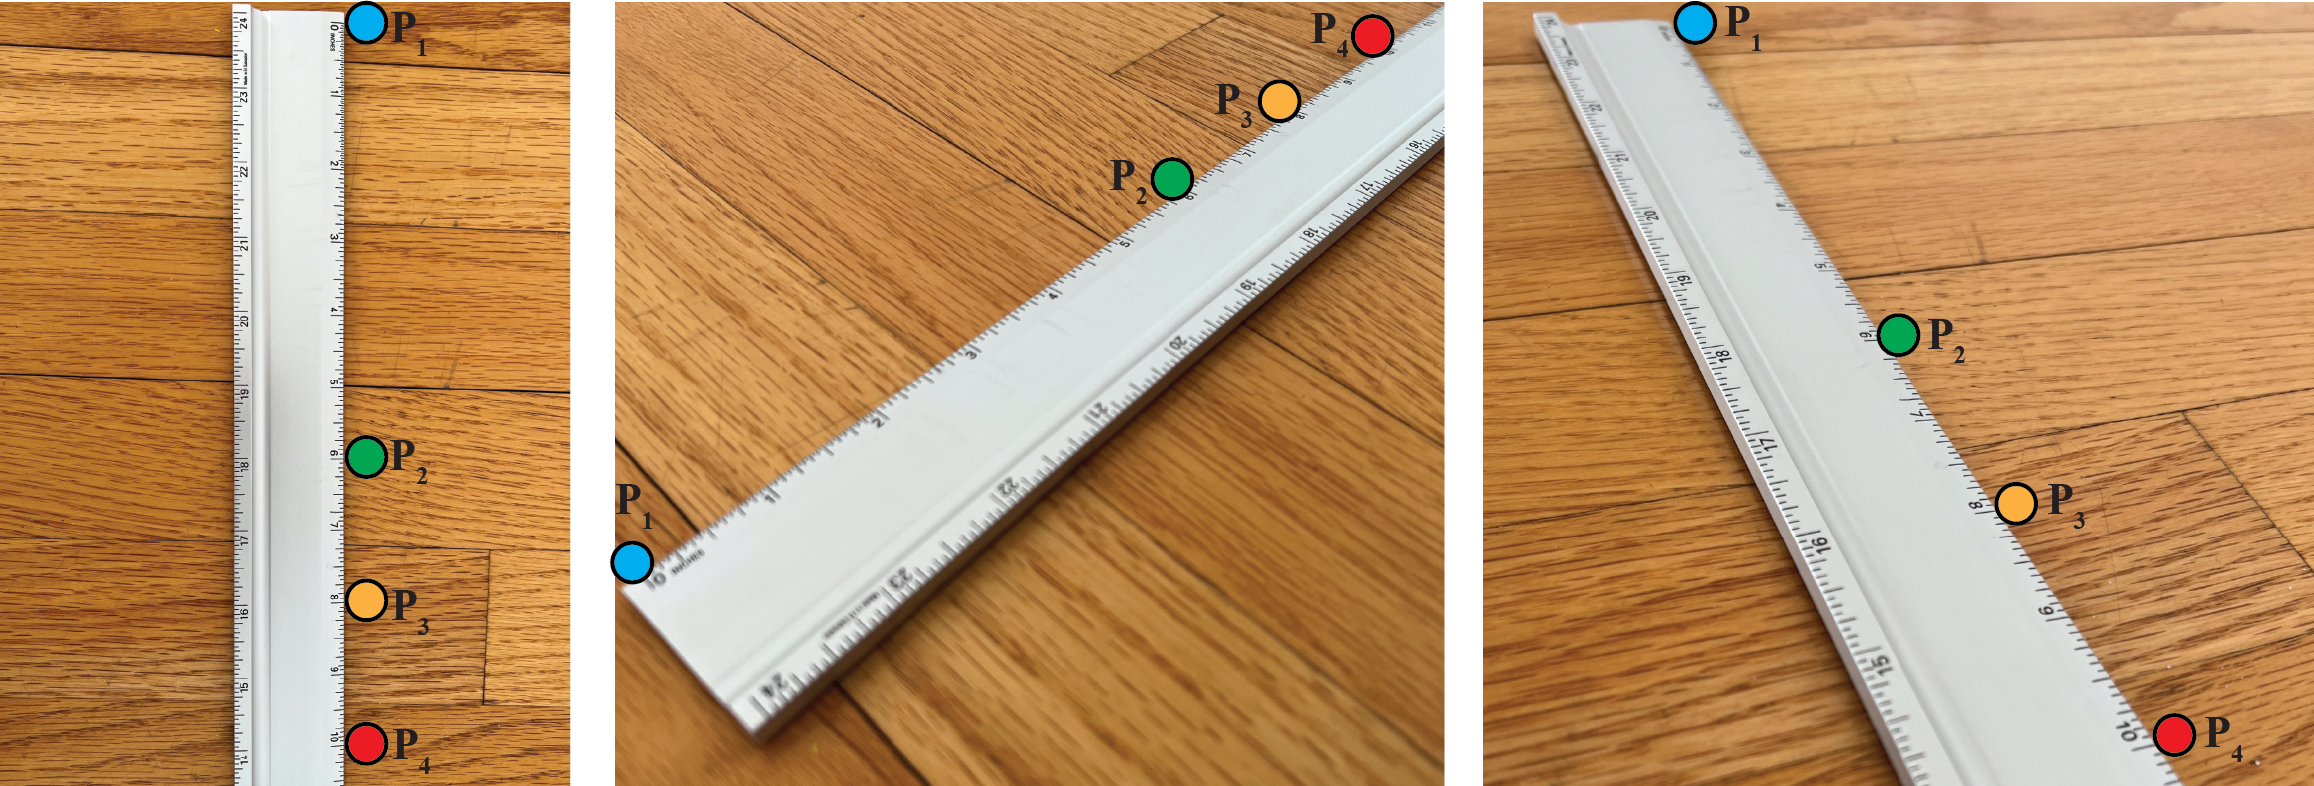
\includegraphics[width=1\linewidth]{figures/single_view_3d/cross-ratio.png}
} 
\caption{Empirical demonstration of the cross-ratio invariant. You can check that measuring distances between the three dots on each image and computing the cross-ratio results in the value 1.6 for the three images.}
\label{fig:cross_ratio_rulers}
\end{figure}

\subsection{Measuring the Height of an Object}

%We will now use the cross ratio to measure 3D distances from a single image. %We will use only the horizon line and the vertical vanishing point of the image and without requiring the projection matrix. 
The problem we will address in this section is how to measure the height of one object given the height of a reference object in the scene. %Let's say we are given the height of the bookshelf as shown in \fig{\ref{fig:office_measuring_desk_setup}}.  Can we estimate the height of the desk?
As shown in \fig{\ref{fig:office_measuring_desk_setup}}, the height of the bookshelf is $h_{\text{bookshelf}}=197$ cm (in this example we will make our measurements using centimeters, but again, the choice of units is not important as long as all the measurements are consistent). Can we use this information together with the geometry of the scene to estimate the height of the desk, $h_{\text{desk}}$?


\begin{figure}
\centerline{
\includegraphics[width=0.8\linewidth]{figures/single_view_3d/office_measuring_desk_setup.eps}
} 
\caption{Given the height of a reference object, the location of the horizon line and one vanishing point, how can we estimate the height of other objects in the scene?}
\label{fig:office_measuring_desk_setup}
\end{figure}

Due to perspective projection, we can not directly compare the relative height of the desk with respect to the height of the bookshelf using distances measured over the image. In order to be able to compare 3D distances using 2D image distances both objects need to be put in correspondence first. The bookshelf height is the distance between the 3D points that correspond to the 2D locations of the bottom of the bookshelf, $\mathbf{g}_b$, and the top of the bookshelf, $\mathbf{t}_b$. Similarly, the desk height is the distance between the 3D points that correspond to $\mathbf{g}_d$ and $\mathbf{t}_d$. We can not use directly the points $\mathbf{g}_b$ and $\mathbf{t}_b$, and  $\mathbf{g}_d$ and $\mathbf{t}_d$ as they are given in image coordinates. In order to be able to use distances in the image domain we need to first translate the points defining the desk height on top of the bookshelf, and then use the cross-ratio invariant to relate the ratio between image distances with the ratios of 3D heights. 

%two lines in the image plane. To compare them, we need to translate one line of top of the other accounting for perspective. 

%The overall algorithm consists in two steps: first, we translate the desk height (i.e, points $\mathbf{g}_d$ and $\mathbf{t}_d$) on top of the bookshelf. Second, we use the cross-ratio to estimate the desk height.  To perform both steps We will only need the location of the horizon line, $\mathbf{h}$, and the position of the vertical vanishing point, $\mathbf{v}_3$, \fig{\ref{fig:office_measuring_desk_sketch}}. 


In the rest, all the vectors refer to image coordinates in homogeneous coordinates. Let's start by projecting the desk height onto the bookshelf. To do this we need to follow several steps: 

\begin{itemize}
\item Estimate the line that passes by the ground points $\mathbf{g}_d$ and $\mathbf{g}_b$. Using homogeneous coordinates, the line can be computed using the cross-product:
\begin{equation}
\boldsymbol{l}_1 = \mathbf{g}_d \times \mathbf{g}_b
\end{equation}

\item Compute the intersection of the line $\boldsymbol{l}_1$ with the horizon line $\mathbf{h}$ as:
\begin{equation}
\mathbf{a} = \boldsymbol{l}_1 \times \mathbf{h} 
\end{equation}
As the line $\boldsymbol{l}_1$ is on the ground plane, the point $\mathbf{a}$ is the vanishing point of line $\boldsymbol{l}_1$.

\item Compute the line that passes by $\mathbf{a}$ and the top of the desk $\mathbf{t}_d$ as:
\begin{equation}
\boldsymbol{l}_2 = \mathbf{a} \times \mathbf{t}_d
\end{equation}
Lines $\boldsymbol{l}_1$ and $\boldsymbol{l}_2$ are parallel on 3D and vertically aligned. 

\item Finally we can compute where line $\boldsymbol{l}_2$ intersects with the bookshelf in the image plane which in this case will also correspond to an intersection of the corresponding 3D lines. We first compute the line that connects the bottom and top points of the bookshelf $\boldsymbol{l}_3 = \mathbf{g}_b \times \mathbf{t}_b$, and now we obtain the intersection with $\boldsymbol{l}_2$ as:
\begin{equation}
\mathbf{b} = \boldsymbol{l}_2 \times \boldsymbol{l}_3 
\end{equation}
\end{itemize}

We can write all the previous steps into a single equation:
\begin{equation}
\mathbf{b} = (((\mathbf{g}_d \times \mathbf{g}_b) \times \mathbf{h}) \times \mathbf{t}_d) \times (\mathbf{g}_b \times \mathbf{t}_b) 
\end{equation}
Point $\mathbf{b}$ is the location where the top of the desk will be if we physically rearrange the furniture to bring the desk and the bookshelf into contact. The segment between points $\mathbf{b}$ and $\mathbf{g}_b$ is the projection of the desk height on the bookshelf. However, due to the foreshortening effect induced by perspective projection, we cannot simply rely on the ratio of image distances to estimate the desk's true height. Instead, we will utilize the cross-ratio invariant to make this estimation. 

\marginnote{As J. J. Gibson pointed out, the ground plane is very useful for all kinds of 3D scene measurements.}[-.2in]


 %We will now make use of the vanishing point to compute the cross-ratio. 
In order to use the cross-ratio invariant we need two sets of four colinear points related by a projective geometry. \Fig{\ref{fig:office_measuring_desk_sketch}} shows a sketch of the setup we have in \fig{\ref{fig:office_measuring_desk}}. 


\begin{figure}[t]
\centerline{
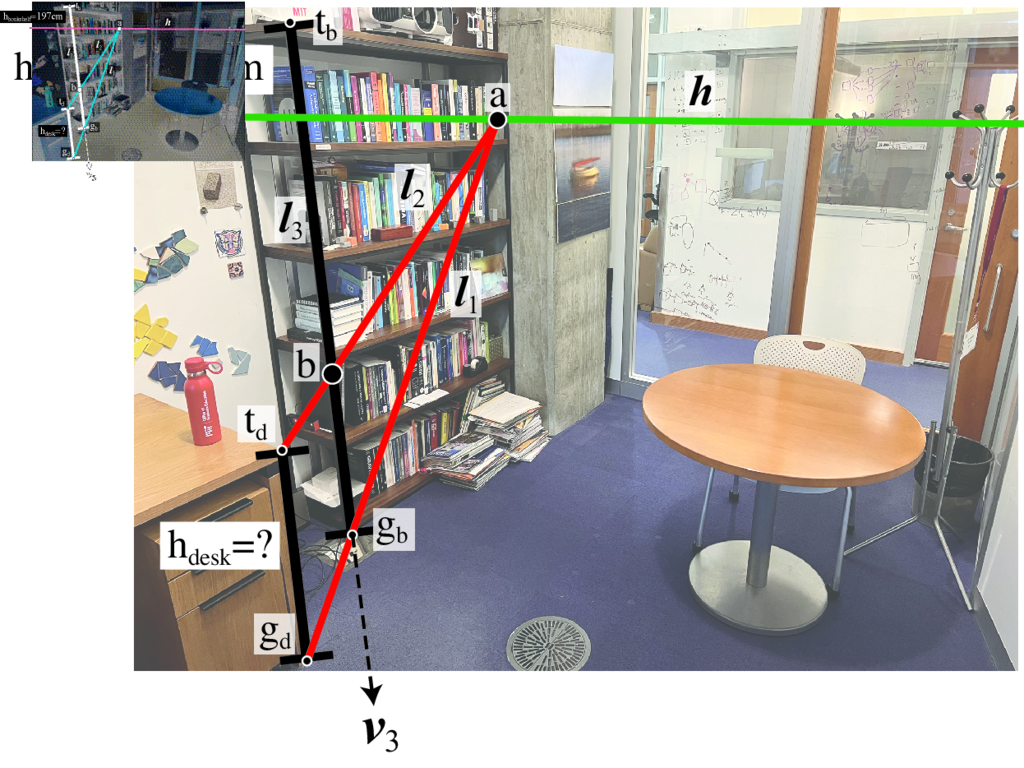
\includegraphics[width=0.85\linewidth]{figures/single_view_3d/office_measuring_desk.eps}
} 
\caption{Projection of desk height onto the bookshelf. We start with the bottom and top image coordinates of points along vertical edges of the bookshelf: 
$\mathbf{t}_b = [702~~2{,}958]^\transpose$ 
$\mathbf{g}_b= [987~~618]^\transpose$ 
and the desk: 
$\mathbf{t}_d = [679~~1{,}018]^\transpose$ 
$\mathbf{g}_d= [793~~59]^\transpose$ 
We compute the points 
$\mathbf{a}= [4{,}471~~2{,}486]^\transpose$ 
and
$\mathbf{b}= [2{,}237~~2{,}765]^\transpose$ 
as described in the text.
}
\label{fig:office_measuring_desk}
\end{figure}


In the image plane, we have the four image points $\mathbf{t}_b$, $\mathbf{b}$, $\mathbf{g}_b$ and $\mathbf{v}_3$. Those four 2D image points correspond to the 3D locations given by the top of the bookshelf, desk height, ground and infinity (which is the location of the vertical vanishing point in 3D).


\begin{figure}
\centerline{
\includegraphics[width=0.7\linewidth]{figures/single_view_3d/office_measuring_desk_sketch.eps}
} 
\caption{Sketch of the setting from \fig{\ref{fig:office_measuring_desk}}. There are two sets of colinear points related by central projection. Their cross-ratios are identical.}
\label{fig:office_measuring_desk_sketch}
\end{figure}

The rest of calculations requires computing distances between points, which only works when using heterogeneous coordinates (or homogeneous coordinates if the last component is equal to 1 for all points). The cross-ratio invariant between both sets of four points gives as the equality:

\begin{equation}
CR(\mathbf{P}_1,\mathbf{P}_2,\mathbf{P}_3,\mathbf{P}_4) = CR(\mathbf{p}_1,\mathbf{p}_2,\mathbf{p}_3,\mathbf{p}_4)
\label{eq:cross_ratio_shelf_desk}
\end{equation}

The left side of the equality corresponds to the distances between the 3D points and the right side to the distances of the image points measured in pixel units. As $\mathbf{P}_1$ is in infinity (as it corresponds to the vanishing point), the left side ratio only has two terms, resulting in the ratio between the bookshelf and desk heights. To compute the hand side we need the coordinates of the corresponding four image points. Those are provided in \fig{\ref{fig:office_measuring_desk}}. Replacing all those values in \eqn{\ref{eq:cross_ratio_shelf_desk}} we obtain:
\begin{equation}
\frac{h_{\text{bookshelf}}}{h_{\text{desk}}} = 
\frac{\left| \mathbf{b} - \mathbf{v}_3 \right| \left| \mathbf{t}_b - \mathbf{g}_b \right| }{\left| \mathbf{b} - \mathbf{g}_b \right| \left| \mathbf{t}_b - \mathbf{v}_3  \right|}
\end{equation}
The only unknown value in this equality is the height of the desk, $h_{\text{desk}}$, which results in $h_{\text{desk}} \simeq 73.1$ cm, which is close to the actual height of the desk (which is around 76 cm).


\marginnote{{\bf Projective invariants} are measures that do not change after perspective projection. The cross-ratio is the most important projective invariant.}

\subsection{Height Propagation to Supported Objects}

The method described in the previous section relies on using vertical lines in contact with the ground plane to propagate information from one point in space to another in order to make measurements. The method can not work if we can not establish the vertical projection of a point into the ground plane (or any other plane of reference). But once we have estimated the height of objects that are in contact with the ground, we can use them to propagate 3D information to other objects not directly on top of the ground. We can estimate the height of objects that are not in contact with the ground if they are on top of objects of known height. As an example, let's estimate the red bottle's height, which we can do after we estimated the height of the desk. 

\Fig{\ref{fig:office_measuring_bottle}} shows how to estimate the height of the bottle. 

\begin{figure}
\centerline{
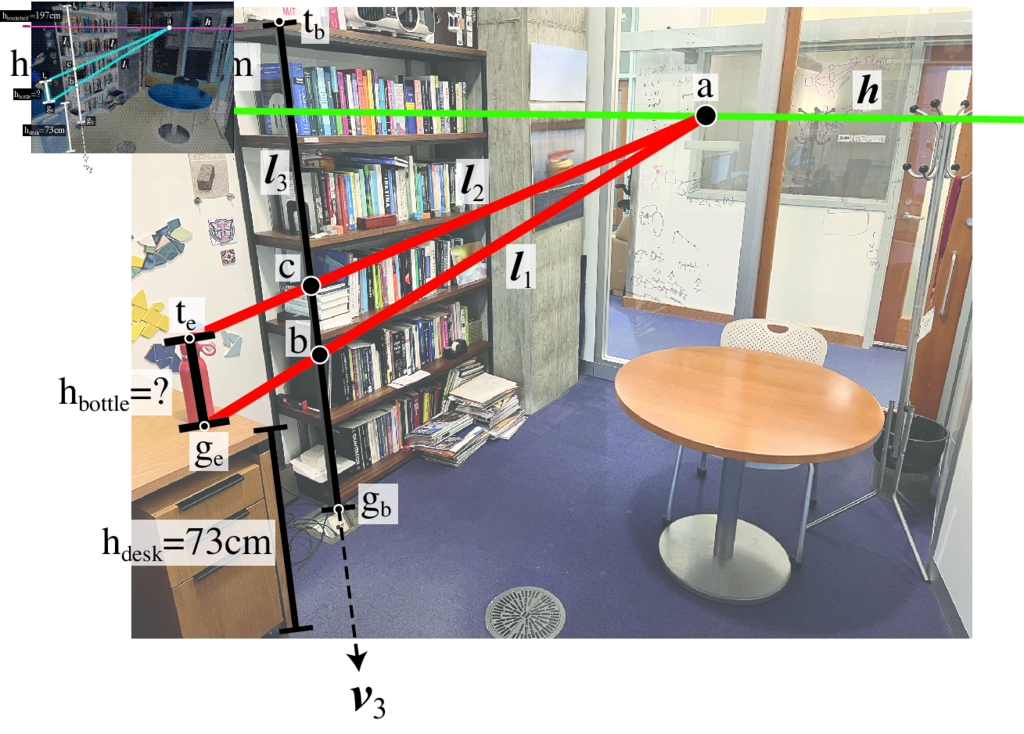
\includegraphics[width=0.85\linewidth]{figures/single_view_3d/office_measuring_bottle.eps}
} 
\caption{Estimating the height of the red bottle. For an object not in the ground we can propagate information from the objects that support it.}
\label{fig:office_measuring_bottle}
\end{figure}

As before, we will project the bottle height on the reference line on the corner of the bookshelf. To do this we need to find two vertically aligned parallel 3D lines that connect the bottle's top and bottom points with the bookshelf. The first line, $\boldsymbol{l}_1$, is the line connecting the bottom of the bottle, $\mathbf{g}_e$, and the point $\mathbf{b}$. These two points are at the same height from the ground plane as $\mathbf{b}$ corresponds to the top of the desk and $\mathbf{g}_e$ is the point of the bottle that is in contact with the top of the desk. The intersection of the line $\boldsymbol{l}_1$ with the horizon line $\mathbf{h}$ give us point $\mathbf{a}$. Connecting point $\mathbf{a}$ with the top of the bottle, point $\mathbf{t}_e$, gives us the second line, $\boldsymbol{l}_2$. The intersection of this line with the reference bookshelf line is the point $\mathbf{c}$. The distance between the point $\mathbf{c}$ and the ground in 3D is the sum  $h_{\text{bookshelf}}+h_{\text{desk}}$. Writing everything into a compact equation results in:
\begin{equation}
\mathbf{c} = (((\mathbf{g}_e \times \mathbf{b}) \times \mathbf{h}) \times \mathbf{t}_e) \times (\mathbf{g}_b \times \mathbf{t}_b) 
\end{equation}
Note that this equation relies on having computed $\mathbf{b}$ first.

Using the cross-ratio invariant we arrive to the following equation:
%\begin{equation}
%\frac{h_{\text{bookshelf}}}{h_{\text{bottle}}+h_{\text{desk}}} = 
%\frac{\left| \mathbf{c} - \mathbf{v}_3 \right| \left| \mathbf{t}_b - \mathbf{g}_b \right| }{\left| %\mathbf{c} - \mathbf{g}_b \right| \left| \mathbf{t}_b - \mathbf{v}_3  \right|}
%\end{equation}
\begin{equation}
h_{\text{bottle}} =
h_{\text{bookshelf}}  \frac{\left| \mathbf{c} - \mathbf{g}_b \right| \left| \mathbf{t}_b - \mathbf{v}_3  \right|}{\left| \mathbf{c} - \mathbf{v}_3 \right| \left| \mathbf{t}_b - \mathbf{g}_b \right| }  - h_{\text{desk}}
\end{equation}
This last equation shows how the height of the bottle is estimated by propagating information from the ground via its supporting object, the desk. Learning based approaches that estimated 3D from single images will have to perform such propagation implicitly. The result that we get is $h_{\text{bottle}} \simeq 27.6$ cm which is close to the real height of 25.5 cm.

This procedure highlights the importance of the correct parsing of the {\bf supported-by hierarchy} between objects in the scene.
\marginnote{A {\bf scene graph} is a representation of a scene using a graph where the nodes correspond to objects, and the edges encode the relationship between them. One important relationship is {\bf supported-by}.}[-.3in]\index{Scene graph}

\section{3D Metrology from a Single View}

In the previous section we showed how to use a reference object to measure other objects. Let's now discuss a more general framework to locate 3D points \cite{criminisi1999accurate}.
%In the office picture from \fig{\ref{fig:vanishing_lines}}, we plotted the world coordinate axis as being aligned with the three dominant orthogonal orientations present in the scene. What the image shows is the projection of the 3D coordinates frame into the image plane. 

The office picture from \fig{\ref{fig:office_world_calibration}} shows the projection of the 3D coordinates frame into the image plane. The axes directions are aligned with the three dominant orthogonal orientations present in the scene and are aligned with the image vanishing points. We will show how can we use the world-coordinates in order to extract 3D object locations from a single image. 


\begin{figure}[t]
\centerline{
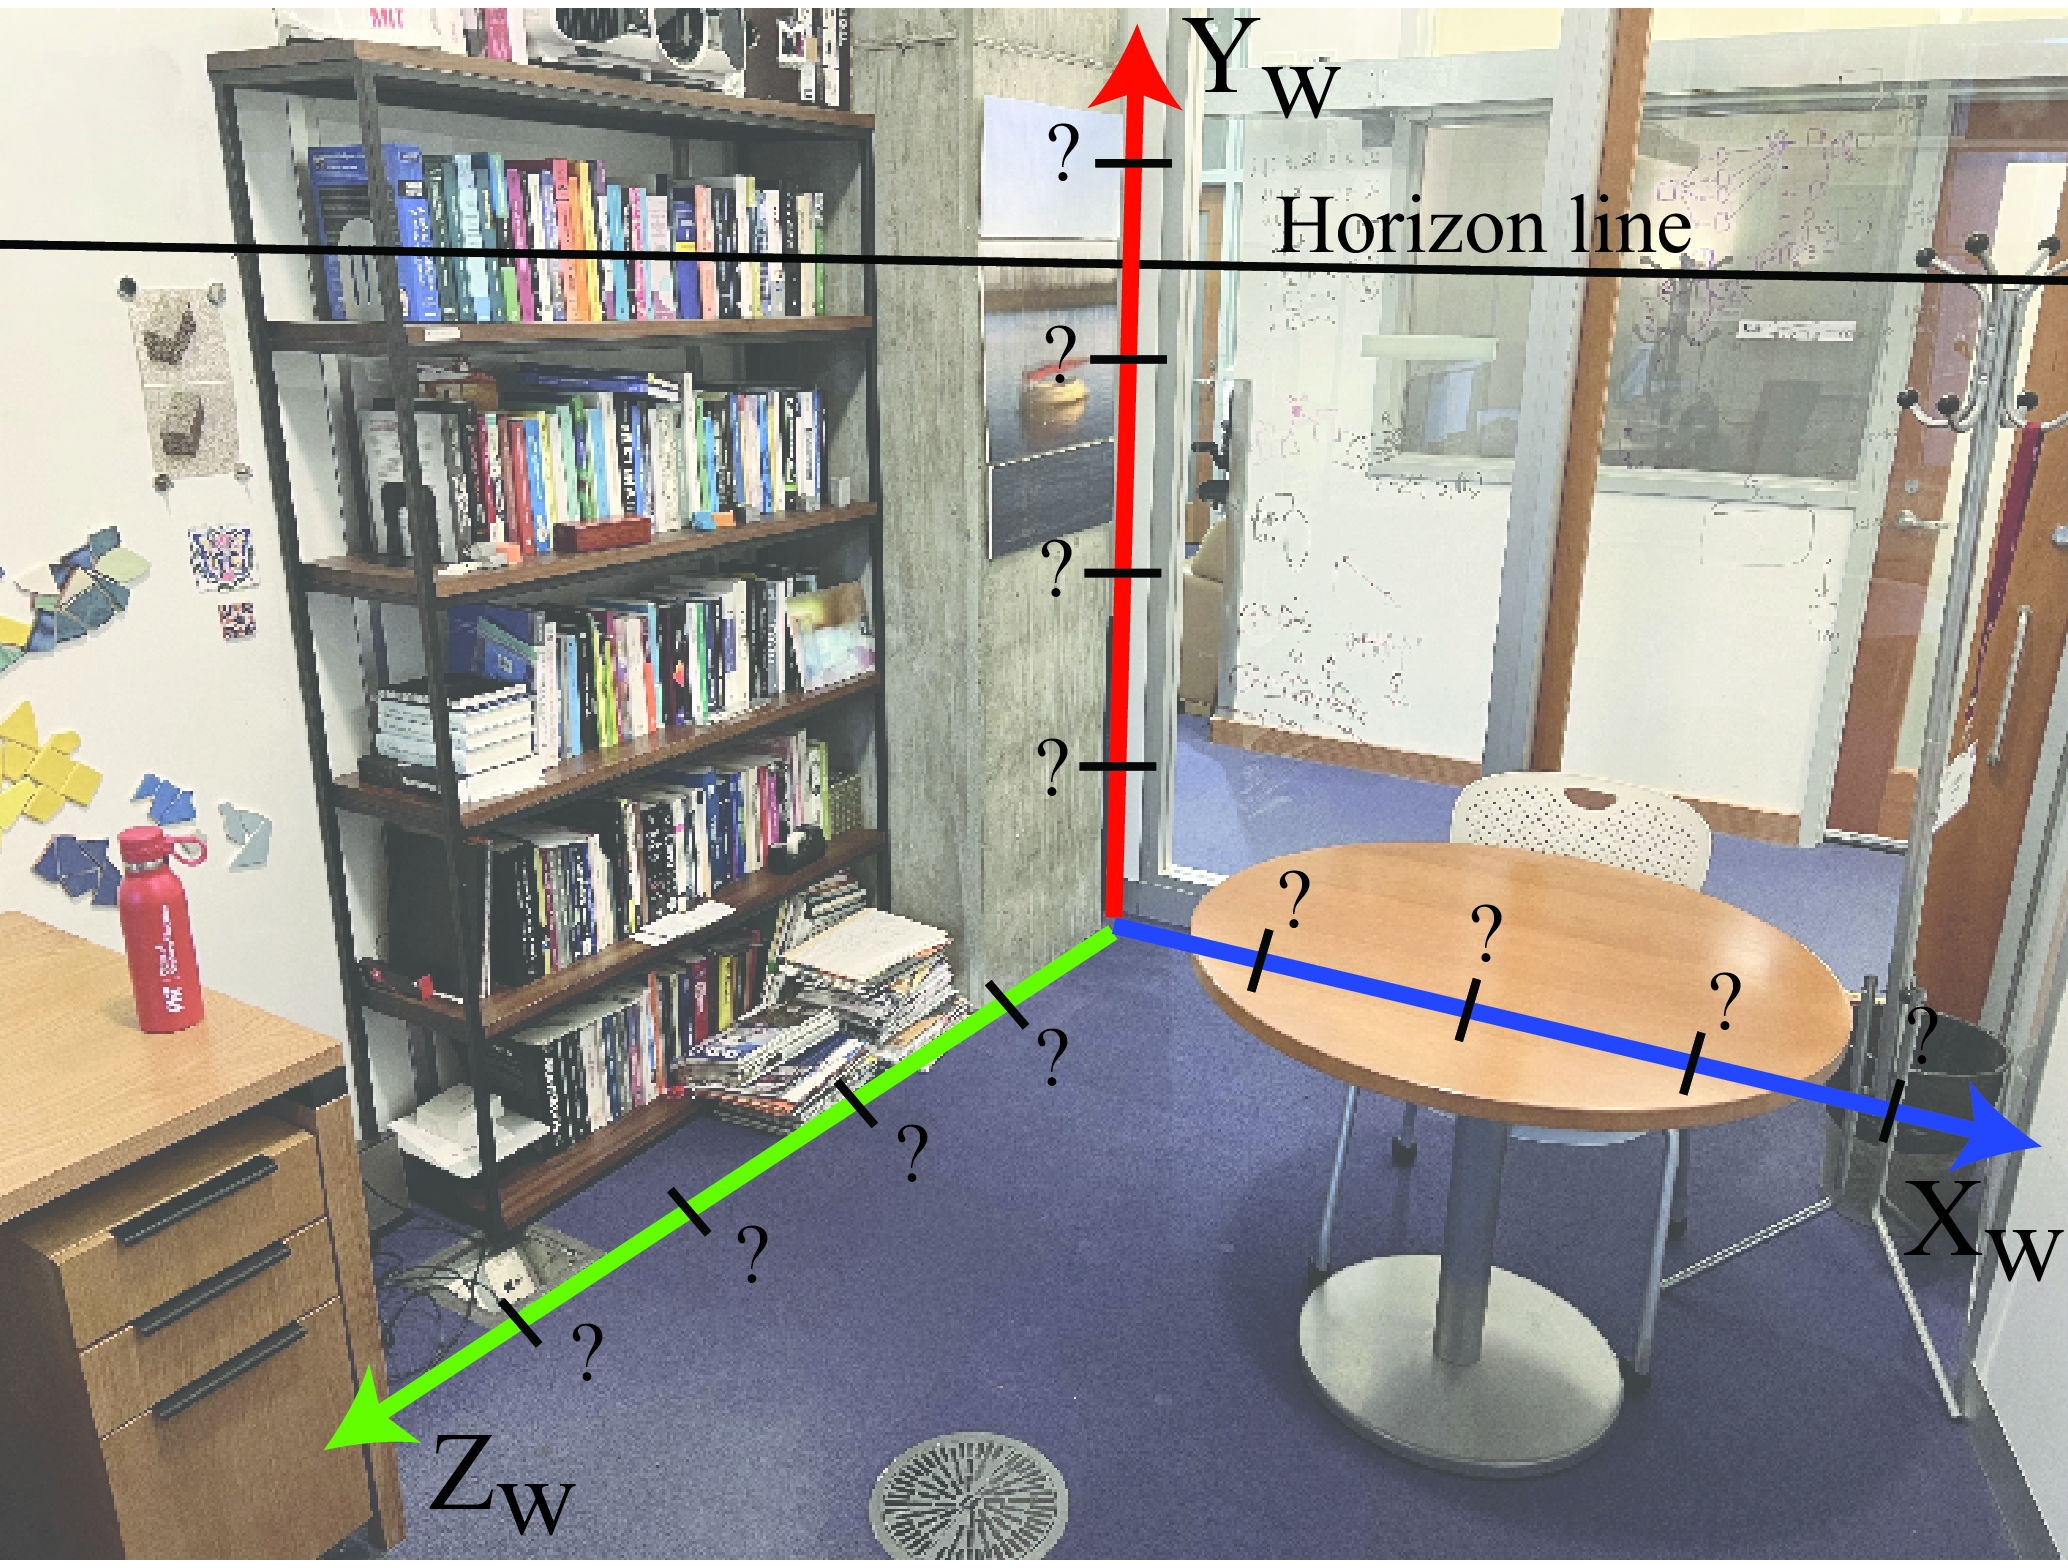
\includegraphics[width=.7\linewidth]{figures/single_view_3d/office_world_calibration.eps}
} 
\caption{Can we find out where to put the ticks in the world-coordinate axes as seen by the camera so that they correspond to calibrated measurements? Simply placing them at evenly spaced intervals along the three axes in the image won't be correct due to perspective projection.}
\label{fig:office_world_calibration}
\end{figure}

In this section we will describe first how to calibrate the projected world-coordinate axes in the image plane and then we will show how to transport points into the 3D world axes in order to measure object sizes and points locations. 
%Where do we place the ticks corresponding to 1, 2, 3, ... meters from the origin on each axis? These points will not be equispaced in the image plane due to the geometric distortion introduced by perspective projection which will distort each axis on a different way.


\subsection{Calibration of the Projected World Axis}

Where should we position the tick marks that correspond to 1, 2, 3, ... meters from the origin on each axis in \fig{\ref{fig:office_world_calibration}}? Simply placing them at evenly spaced intervals along the axis in the image won't be correct. Due to geometric distortion introduced by perspective projection, the tick marks are not evenly spaced within the image plane. This distortion affects each axis in a distinct manner.

Let's start assuming we know the location of some arbitrary 3D distance to the origin on each axis that we will denote by $\alpha_X$, $\alpha_Y$ and $\alpha_Z$. The question is, where do we place the ticks for $k\alpha_X$, $k\alpha_Y$ and $k\alpha_Z$ for all $k$? We will use the cross-ratio to calibrate the projection of the world coordinate system in the image plane. For doing this we will need the location of the horizon line of a reference plane (i.e. the ground plane), the position of the orthogonal vanishing point and the real measure of one object in the scene. 


As shown in \fig{\ref{fig:axis_calibration_procedure}}{a} we can use the cross-ratio to estimate the location of the points $Y= k \alpha_X$ where $\alpha_X$ is an arbitrary constant as shown in \fig{\ref{fig:axis_calibration_procedure}}{b}, and the corresponding image location $r$, for $k=1$, is chosen arbitrarily as shown in \fig{\ref{fig:axis_calibration_procedure}}{a}. Due to perspective projection, the image projection of the point $Y= k \alpha_X$ will not be evenly spaced in the image.  In this particular example we chose the orientation of the world axis in image coordinates to be aligned with the location of the vanishing points.

\begin{figure}[t]
\centerline{
\includegraphics[width=1\linewidth]{figures/single_view_3d/axis_calibration_procedure.eps}
} 
\caption{Using the cross-ratio invariant to project the world coordinates into the image using only the vanishing points.}
\label{fig:axis_calibration_procedure}
\end{figure}

In order to calibrate the axis we need to know the dimensions of an object in the scene. We need measurements along the three axis. In this example, we used the bookshelf height (197 cm) and the radius of the table base (50 cm). Using these reference measurements we can 
solve for the image locations of the ticks $\alpha_X=\alpha_Y=\alpha_Z=1$ m. 

\Fig{\ref{fig:office_all_calibrated_box}} shows the final calibrated axes with ticks placed each 50 cm along each of the three axes.  


%\begin{figure}
%\centerline{
%\includegraphics[width=1\linewidth]{figures/single_view_3d/axis_calibration.eps}
%} 
%\caption{Projecting an object height into the $Y$ axis.}
%\label{fig:axis_calibration}
%\end{figure}


\begin{figure}[t]
\centerline{
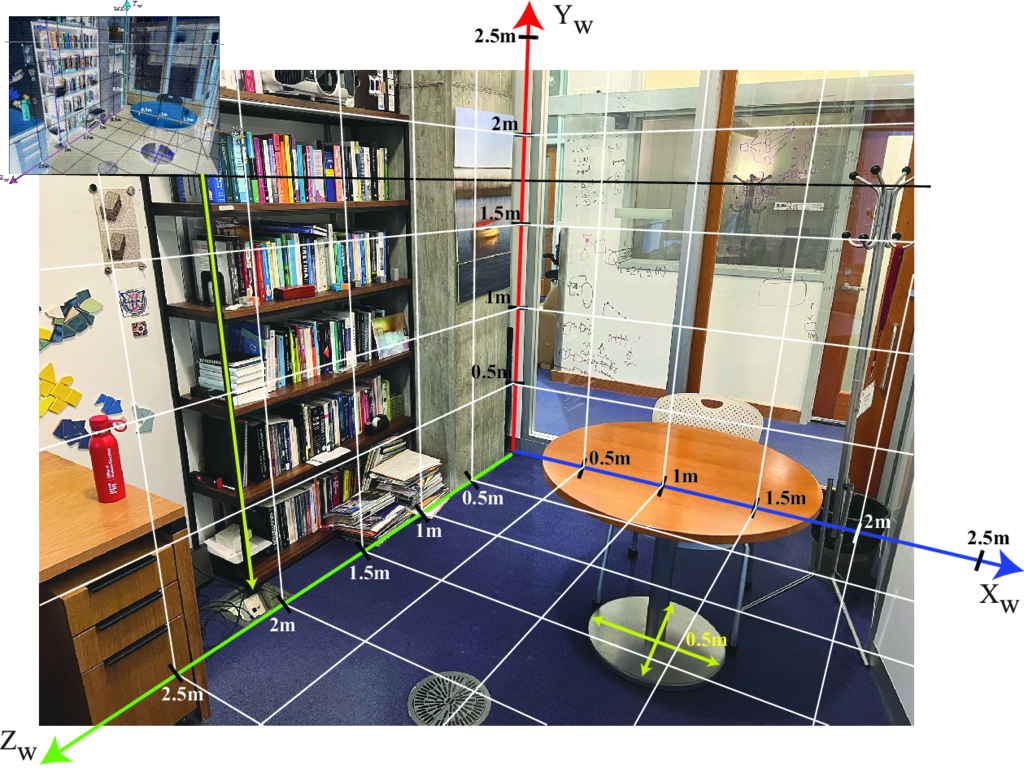
\includegraphics[width=1\linewidth]{figures/single_view_3d/office_all_calibrated_box.eps}
} 
\caption{Calibrated world axes. Each axis is calibrated using the measurement of a scene element parallel to the world-coordinate axis. In this example, we used the bookshelf height (197 cm) and the radius of the table base (50 cm). From the calibrated axes, you can see that the office is around 250 cm wide.}
\label{fig:office_all_calibrated_box}
\end{figure}

From this calibrated system we can directly read the height of the camera. The location of the camera coincides with the location of the horizon line because, in this example, the ground plane is horizontal. It seems that the center of the camera is approximately 163 cm above the ground.


There are many ways in which we can arrive to the same result. 


\subsection{Locating a 3D Point}

%\fig{\ref{fig:locating_a_3d_point}}{a} shows a 3D point $\mathbf{P}$. The world coordinate system is calibrated following the procedure described in the previous section. 


In the absence of any other information, we can not recover the 3D location of a single point $\mathbf{P}$ from a single view as illustrated in \fig{\ref{fig:locating_a_3d_point}}{a}. But real world scenes are composed by a multitude of objects providing context, which allows solving the 3D estimation problem even with just a single image. In the previous section we showed how to estimate the height of an object, here we show how to estimated the 3D coordinates of a point. 

The basic procedure is illustrated in \fig{\ref{fig:locating_a_3d_point}}{b}. The trick consists in using context (what object is the point part of, where is the horizon line of the scene and where are the vanishing points) to estimate 3D from a single image. It suffices to know that the point $\mathbf{P}$ belongs to an object that is in contact with the ground and the geometry of this object provides the information to localize the projection of the point $\mathbf{P}$ on the ground plane, which we denote with $\mathbf{G}$. 

\begin{figure}
\centerline{
\includegraphics[width=1\linewidth]{figures/single_view_3d/locating_a_3d_point.eps}
} 
\caption{(a) In the absence of any other information, we can not recover the 3D location of point $\mathbf{P}$. (b) If we are given a way to project the point P into the ground, then we can read out the coordinates of the point by projecting into the world axis.}
\label{fig:locating_a_3d_point}
\end{figure}

Once we know the image location of the projection of the 3D point $\mathbf{P}$ to the ground, $\mathbf{G}$, we can project this point to the world-coordinate axis. To estimate the $Y$-coordinate we use a similar method as the one described in the previous section. We first find the line, $\boldsymbol{l}_3$,  that passes by the point $\mathbf{G}$ and the origin, and then find the intersection with the horizon line, giving the point $\mathbf{v}$. Next, find the line, $\boldsymbol{l}_4$, that passes by $\mathbf{v}$ and $\mathbf{P}$. The intersection of $\boldsymbol{l}_4$ with the $Y_w$-axis gives the coordinate $P_y$. The $P_x$ and $P_z$ coordinates can be obtained by connecting $\mathbf{G}$ with the vanishing points $\mathbf{v}_1$ and $\mathbf{v}_2$.

Here we have been using the ground plane as a reference. But the same idea can be applied if we know the projection of the point $\mathbf{P}$ into another plane with a known horizon line.

In summary, we can recover the location of the 3D point from a single image by propagating information from the calibrated world-coordinate axis using the vanishing points that are aligned with the axis.  


%\subsection{Recovering the office measurements}


\section{Camera Calibration from Vanishing Points}
%~\\
% http://www.bmva.org/bmvc/1999/papers/38.pdf
% https://www.cs.princeton.edu/courses/archive/fall13/cos429/lectures/11-epipolar
In the previous chapters, we have seen different methods to calibrate a camera. We saw that we could do it by taking pictures of a calibration pattern, and we also showed that we can extract both the intrinsics and extrinsics from a set of  3D points and their image correspondences. Here we will see a different method that uses only the vanishing points to extract the camera parameters; note that this method will only work under some conditions.

The first step consists in finding the vanishing points in the image. Let's use the office picture from \fig{\ref{fig:vanishing_lines}}. In this particular scene there are many parallel lines in 3D, and they also happen to be parallel to the three directions we used to define the world coordinates system. Therefore, the three vanishing points are also aligned with the world coordinate axis. 



Let's assume that we have three orthogonal vanishing directions. That is the vectors $\mathbf{D}_1$, $\mathbf{D}_2$, and $\mathbf{D}_3$ are orthogonal in 3D. From \eqn{\ref{eq:vanishing_projection}}, the vanishing points measured on the image are the result of projecting $\mathbf{D}_1$, $\mathbf{D}_2$, and $\mathbf{D}_3$ into the image using the unknown camera projection matrix. We will use the vanishing points to derive a set of constraints on the projection matrix. To do this, we start by inverting \eqn{\ref{eq:vanishing_projection}}:
\begin{equation}
\mathbf{D}_i = \mathbf{R}^{-1} \mathbf{K}^{-1} \mathbf{v}_i
\label{eq:vanishing_projection_inv}
\end{equation}
Because the vectors $\mathbf{D}_i$ are orthogonal, we have that $\mathbf{D}_i^{\transpose} \mathbf{D}_j = 0$ for $i \neq j$. Therefore, we can write:
\begin{equation}
\mathbf{D}_i^\transpose \mathbf{D}_j = \mathbf{v}_i^\transpose \mathbf{K}^{-\transpose} \mathbf{R}^{-\transpose} \mathbf{R}^{-1} \mathbf{K}^{-1} \mathbf{v}_j 
\label{eq:vanishing_projection_constraint}
\end{equation}
As $\mathbf{R}$ is an orthonormal matrix, we have that $\mathbf{R}^{-\transpose} \mathbf{R}^{-1} = \mathbf{I}$, resulting in a relationship that only depends on the intrinsic camera parameters $\mathbf{K}$:
\begin{equation}
\mathbf{D}_i^T \mathbf{D}_j = \mathbf{v}_i^\transpose \mathbf{K}^{-\transpose} \mathbf{K}^{-1} \mathbf{v}_j = 0
\label{eq:vanishing_projection_constraint}
\end{equation}


It is useful to define the following matrix:
\begin{equation}
\mathbf{W} =  \mathbf{K}^{-\transpose} \mathbf{K}^{-1}
\end{equation}
This is also known as the {\bf conic matrix}
\index{Conic matrix}
and it has lots of different properties \cite{Hartley2004}. 
\marginnote{The intrinsic camera parameter matrix is:
\begin{equation*}
\mathbf{K} = 
    \begin{bmatrix}
    a & 0 & c_x\\
    0 & a & c_y\\
    0 & 0 & 1
    \end{bmatrix}
\end{equation*}

Its inverse has a simple structure:
\begin{equation*}
\mathbf{K}^{-1} = 
    \begin{bmatrix}
    \frac{1}{a} & 0 & -\frac{c_x}{a}\\
    0 & \frac{1}{a} & -\frac{c_y}{a}\\
    0 & 0 & 1
    \end{bmatrix}
\end{equation*}
}[-1.5in]

If we assume that the skew parameter of the intrinsic camera matrix is zero, then the matrix $\mathbf{W}$ has a very particular structure and it has only four different values:
\begin{equation}
\mathbf{W} = 
    \begin{bmatrix}
    a & 0 & b\\
    0 & a & c\\
    b & c & d
    \end{bmatrix}
\end{equation}
Using \eqn{\ref{eq:vanishing_projection_constraint}}, we can derive a linear constraint on the values $a,b,c,d$ for each pair of vanishing points. Defining the vector $\mathbf{w}=[a~b~c~d]^\transpose$, we can rewrite \eqn{\ref{eq:vanishing_projection_constraint}} into a system of linear equations that has the form:
\begin{equation}
\mathbf{A} \mathbf{w} = 0
\end{equation}


The linear equation can be solved with the singular value decomposition (SVD) and the result is the eigenvector with the smallest eigenvalue. 

Once we have $\mathbf{W}$, we can find $\mathbf{K}$ by using the Cholesky factorization, which decomposes a matrix as the product of an upper triangular matrix and its transpose. The last step is to normalize the result by normalizing all the matrix values so that the value on the bottom-right side is 1.  In our running example of the office picture, we get the following solution for $\mathbf{K}$:
\begin{equation}
    \mathbf{K} = 
    \begin{bmatrix}
    3{,}054.6    &      0    &     1{,}999.4\\
       0    &       3{,}054.6    &     1{,}528.3\\
       0    &          0    &          1
    \end{bmatrix}
\end{equation}

\marginnote{The Cholesky factorization of an Hermitian positive-definite matrix, $\mathbf{A}$, is $\mathbf{A} = \mathbf{B}\mathbf{B}^\transpose$, 
where $\mathbf{B}$ is a lower triangular matrix with positive diagonal values. The factorization is unique.
}[-1.25in]


We can now compare this result with the one we obtained when we (1) used the physical camera parameters (\sect{\ref{sec:simple_unreliable_calibration_method}}); (2) used a calibration pattern (\sect{\ref{sec:simple_unreliable_calibration_method}}); and (3) used a collection of 3D points and the corresponding image locations (\sect{\ref{sec:a_toy_example}}). We can see that in all cases we get similar results, although, not identical. 

% Can we recover the camera rotation and location with respect to world coordinates?



\section{Concluding Remarks}

In this chapter we have shown how to use geometric image features (vanishing points, horizon line) and projective invariants (such as the cross-ratio) to estimate 3D scene properties from a single image. However, most of the steps required some manual intervention. All of those steps can be performed in a fully automatic way by training detectors to localize the full extend of an object as we will discuss in \chap{\ref{chapter:object_recognition}} and detecting points of contact between objects. 

One of the key insights from this chapter is that a single images contain a lot of information that, in most cases, is enough to estimate metric 3D information from a single 2D image. In the next chapter we will discuss learning-based methods for 3D estimation from images. 